%%%%%%%%%%%%%%%%%%%%%%%%%%%%%%%%%%%%%%%%%
% Short Sectioned Assignment LaTeX Template Version 1.0 (5/5/12)
% This template has been downloaded from: http://www.LaTeXTemplates.com
% Original author:  Frits Wenneker (http://www.howtotex.com)
% License: CC BY-NC-SA 3.0 (http://creativecommons.org/licenses/by-nc-sa/3.0/)
%%%%%%%%%%%%%%%%%%%%%%%%%%%%%%%%%%%%%%%%%

%----------------------------------------------------------------------------------------
%	PACKAGES AND OTHER DOCUMENT CONFIGURATIONS
%----------------------------------------------------------------------------------------

\documentclass[paper=a4, fontsize=11pt]{scrartcl} % A4 paper and 11pt font size

% ---- Entrada y salida de texto -----

\usepackage[T1]{fontenc} % Use 8-bit encoding that has 256 glyphs
\usepackage[utf8]{inputenc}
%\usepackage{fourier} % Use the Adobe Utopia font for the document - comment this line to return to the LaTeX default

% ---- Idioma --------

\usepackage[spanish, es-tabla]{babel} % Selecciona el español para palabras introducidas automáticamente, p.ej. "septiembre" en la fecha y especifica que se use la palabra Tabla en vez de Cuadro

% ---- Otros paquetes ----

\usepackage{url} % ,href} %para incluir URLs e hipervínculos dentro del texto (aunque hay que instalar href)
\usepackage{hyperref}
\hypersetup{
	colorlinks=true,
	linkcolor=black,
	urlcolor=black,
	citecolor=black,
}
\usepackage{amsmath,amsfonts,amsthm} % Math packages
%\usepackage{graphics,graphicx, floatrow} %para incluir imágenes y notas en las imágenes
\usepackage{graphics,graphicx, float} %para incluir imágenes y colocarlas

% Para hacer tablas comlejas
%\usepackage{multirow}
%\usepackage{threeparttable}

%\usepackage{sectsty} % Allows customizing section commands
%\allsectionsfont{\centering \normalfont\scshape} % Make all sections centered, the default font and small caps

\usepackage{fancyhdr} % Custom headers and footers
\pagestyle{fancyplain} % Makes all pages in the document conform to the custom headers and footers
\fancyhead{} % No page header - if you want one, create it in the same way as the footers below
\fancyfoot[L]{} % Empty left footer
\fancyfoot[C]{} % Empty center footer
\fancyfoot[R]{\thepage} % Page numbering for right footer
\renewcommand{\headrulewidth}{0pt} % Remove header underlines
\renewcommand{\footrulewidth}{0pt} % Remove footer underlines
\setlength{\headheight}{13.6pt} % Customize the height of the header

\numberwithin{equation}{section} % Number equations within sections (i.e. 1.1, 1.2, 2.1, 2.2 instead of 1, 2, 3, 4)
\numberwithin{figure}{section} % Number figures within sections (i.e. 1.1, 1.2, 2.1, 2.2 instead of 1, 2, 3, 4)
\numberwithin{table}{section} % Number tables within sections (i.e. 1.1, 1.2, 2.1, 2.2 instead of 1, 2, 3, 4)

\setlength\parindent{0pt} % Removes all indentation from paragraphs - comment this line for an assignment with lots of text

\newcommand{\horrule}[1]{\rule{\linewidth}{#1}} % Create horizontal rule command with 1 argument of height
\usepackage{booktabs}

\usepackage{listings}
\usepackage{color}
\usepackage{xcolor}
\lstdefinestyle{customc}{
	belowcaptionskip=1\baselineskip,
	breaklines=true,
	frame=L,
	xleftmargin=\parindent,
	language=C,
	showstringspaces=false,
	basicstyle=\footnotesize\ttfamily,
	keywordstyle=\bfseries\color{green!40!black},
	commentstyle=\itshape\color{purple!40!black},
	identifierstyle=\color{blue},
	stringstyle=\color{orange},
}

\lstset{escapechar=@,style=customc}
\usepackage{url}

\title{	
	\normalfont \normalsize
	\begin{figure}[htb]
		\centering
		
\includegraphics[width=0.3\textwidth]{./imagenes/1}
	\end{figure}
	\textsc{\textbf{Inteligencia de Negocio} \\ Grado en Ingeniería Informática \\ Universidad de Granada \\
	Curso 2018-2019} \\ [25pt] % Your university, school and/or department name(s)
	\begin{figure}[htb]
		\centering
		
\includegraphics[width=0.15\textwidth]{./imagenes/2}
	\end{figure}
	\horrule{0.5pt} \\[0.4cm] % Thin top horizontal rule
	\huge Memoria Práctica 2. Grupo 1 \\
	\huge Segmentación para Análisis Empresarial.
	\\ % The assignment title
	\horrule{2pt} \\[0.5cm] % Thick bottom horizontal rule
}
\author{Félix Ramírez García  \\
\href{mailto:felixramirezgarcia@correo.ugr.es}{felixramirezgarcia@correo.ugr.es}} % Nombre y apellidos
\date{\normalsize\today} % Incluye la fecha actual

%----------------------------------------------------------------------------------------
% DOCUMENTO
%----------------------------------------------------------------------------------------

\begin{document}
	
	\maketitle % Muestra el Título
	
	\newpage %inserta un salto de página
	
	\tableofcontents % para generar el índice de contenidos
	
	\listoffigures % para generar índice de imágenes.
	
	\listoftables % para generar índice de tablas.
	
	\newpage

	%----------------------------------------------------------------------
	%							Introducción
	%----------------------------------------------------------------------	
	
	\section[Introducción]{Introducción.}

	Esta practica ha sido llevada a cabo para la asignatura Inteligencia del Negocio de cuarto
	curso de Ingeniería Informática de la Universidad de Granada. Veremos el uso de algoritmos de aprendizaje
	no supervisado de agrupamiento para el análisis empresarial.\\

	Vamos a trabajar con el conjunto de datos publicados en el ultimo censo de población realizado por 
	el Instituto Nacional de Estadística (INE) en 2011 \cite{cite1}. \\

	Mediante las distintas variables categóricas (estado civil, sexo,
	,etc..) se van a fijar tres casos de estudio donde centrar el análisis. \\

	Para realizar la practica se ha usado el lenguaje de programación Phyton en la versión 3.7 \cite{cite2}
	y se han utilizado los siguientes algoritmos de clustering: \\

	K-means  \cite{cite3} \\
	Spectral clustering \cite{cite5} \\
	Mean Shift \cite{cite6} \\
	Ward \cite{cite7} \\
	Birch \cite{cite9} \\

	El conjunto de datos extraídos del INE cuenta con un total de 83.499 casos ,identificados 
	cada uno por 142 variables , del cual se seleccionan subconjuntos de datos para los casos de 
	estudio que se presentan posteriormente.\\

	En esta practica se abordara el problema haciendo un estudio que se reflejara en varias gráficas
	y tablas con datos estadísticos la mayor cantidad de información posible.\\

	Por último se extraerán conclusiones finales apropiadas para cada caso de estudio. En particular
	se usaran un total de 5 algoritmos de clustering, para los cuales se analizaran varias métricas y gráficas
	para analizar los resultados obtenidos.

	%----------------------------------------------------------------------
	%							Casos de estudio
	%----------------------------------------------------------------------	

	\section[Casos de estudio]{Casos de estudio.}

	Dentro de este apartado, se realizaran 3 casos de estudio, en cada uno de ellos se ejecutaran los 5 algoritmos
	de clustering seleccionados y se calcularan las métricas y gráficas para su posterior análisis.\\

	Las métricas usadas para comparar los datos son: numero de clusters, indice Calinski-Harabaz, la métrica
	Silhouete y el tiempo de ejecución de cada algoritmo. Las gráficas son ScatterMatrix , HeatMap , Dendograma y HeatMap con Dendograma.

	%----------------------------------------------------------------------
	%							Caso de estudio 1
	%----------------------------------------------------------------------	

	\subsection[Caso de estudio 1. Personas que viven con personas mayores de 65 años]{Primer caso de estudio: Personas que viven con personas mayores de 65 años}

	En este primer caso de estudio nos vamos a centrar en familias que viven en su hogar con personas mayores , analizaremos el numero de personas
	dentro del hogar y que rango de edades tienen.
	Las variables que vamos a utilizar son : \\

	HM5 : Número de personas de 0 a 4 años en el hogar \\
	H0515 : Número de personas de 5 a 15 años en el hogar  \\
	H1624 : Número de personas de 16 a 24 años en el hogar  \\
	H2534  : Número de personas de 25 a 34 años en el hogar \\
	H3564 : Número de personas de 35 a 64 años en el hogar   \\

	En la siguiente tabla se muestran los datos asociados a cada algoritmo usado para este caso de estudio
	de personas que viven con personas mayores , datos como el numero de clusters que se han usado,
	la metrica Calinski-harabasz (CH) , la metrica Siljouette (SC) y el tiempo en segundos que ha tardado
	el algoritmo para ejecutarse . Para este caso de estudio se han contado con un total de 23897 instancias.\\

	\begin{table}[htbp]
		\begin{center}
			\begin{tabular}{c | c | c | c | c}
				\toprule
				Algoritmo &  N Clusters &     HC metric &  SC metric &        Time \\
				\midrule
				K-means   &           4 &  29697.858169 &   0.764292 &    0.100956 \\
				Birch     &           6 &  21480.901579 &   0.729611 &    0.646720 \\
				Ward      &          10 &  33361.232561 &   0.845975 &   19.899369 \\
				MeanShift &          14 &  32215.188490 &   0.855566 &    0.784660 \\
				Spectral  &           3 &  26907.715611 &   0.726861 &  421.776694 \\
				\bottomrule
			\end{tabular}
		\end{center}
	\end{table}

	Para la realización de las tablas del estilo de la anterior se ha usado el siguiente código python: \\

	\lstset{language=python}
	\begin{lstlisting}[frame=single]
def createLatexDataFrame(data):
	my_index = list(dict(data.items()).keys())
	my_data = list(data.values())
	my_cols = list(my_data[0].keys())
	latexDF = pd.DataFrame()

	for row in range(len(my_index)):
		aux = pd.DataFrame(data=my_data[row],index=[my_index[row]],columns=my_cols)
		latexDF = pd.concat([latexDF,aux])

	return latexDF

for algorithm_name,algorithm in clustering_algorithms:
    results = dict()
    met, clusterFrame, timeAlg,cluster_predict = createPrediction(dataframe=X, data=X_normal, model=algorithm)
    n_clusters=len(set(cluster_predict))

    if( n_clusters > 15 ):
        X_filtrado = clusterFrame[clusterFrame.groupby('cluster').cluster.transform(len) > min_size]
    else:
        X_filtrado = clusterFrame

    makeScatterMatrix(data=X_filtrado,outputName="./imagenes/scatterMatrix_caso1_" +algorithm_name,displayOutput=False)
    makeHeatmap(data=X_filtrado,outputName="./imagenes/heatmap_caso1_"+algorithm_name,displayOutput=False)
    makeDendograma(data=X_filtrado,outputName="./imagenes/dendograma_caso1_"+algorithm_name,displayOutput=False)
    makeHeatMapConDendograma(data=X_filtrado,outputName="./imagenes/heatmapcondendograma_caso1_"+algorithm_name,displayOutput=False)
    
    results['N Clusters']=n_clusters
    results['HC metric']=met[0]
    results['SC metric']=met[1]
    results['Time']=timeAlg

    outputData[algorithm_name] = results

latexCaso1 = createLatexDataFrame(data=outputData)
	\end{lstlisting}

	En cada caso de estudio nos encontramos con una tabla como la anterior , que nos permitirá valorar 
	los algoritmos y parámetros usados. \\

	En este caso , vemos como para el indice Calinski-Harabasz hay tres algoritmos que están en cabeza (K-means, Ward, MeanShift), ya que 
	el indice CH se define como la razón entre la dispersión interior de los clusters y la dispersión entre clusters , 
	, el objetivo es maximizar este indice. Básicamente viene a reflejar una de las máximas de los algoritmos de clustering
	, y es que un buen metodo de clustering debe maximizar la similaridad intra-clusters y minimizar la similaridad
	inter-cluster. De esta forma podemos decir que estos tres son los que mejor comportamiento tienen. Ya que se encuentra muy lejos del algoritmo
	Spectral. \\

	Para el indice Silhouette no ocurre lo mismo que para el Calinski-Harabasz, ya que todos los resultados se encuentra a la par,
	teniendo MeanShift la mejor métrica de los
	5 algoritmos pero no por mucho. El indice Silhouette mide como de compactos y separados están los clusters, el intervalo de este 
	indice esta entre -1 y 1 , donde los valores cercanos a -1 tienen una mala agrupacion , y los valores cercanos a 1 
	tienen una buena agrupación.\\
	
	Quedando los algortimos Ward y MeanShift como los que mejores se comportan podríamos clonar el numero de clusters usados en ese algoritmo 
	para ver si se producen mejoras en las métricas de los demás algoritmos , esto lo abordaremos mas adelante.\\

	Por ultimo cabe decir que el algoritmo Spectral es que mayor tiempo de ejecución tiene. En las siguientes subsecciones
	se muestran gráficas y tablas de algoritmos asociadas a cada algoritmo usado para cada caso de estudio
	, y al final exponemos un análisis de los resultados obtenidos.\\

	Cabe destacar que se ha realizado la eliminación de aquellos clusters con pocos datos (ouliers) . Se ha realizado mediante un 
	filtrado a los clusters con menos de 5 elementos. \\

	%----------------------------------------------------------------------
	%							k-means caso 1
	%----------------------------------------------------------------------	

	\subsubsection{Resultados algoritmo K-Means caso 1}

	El algoritmo K-means es uno de los mas simples de todos los algoritmos de aprendizaje no supervisado. 
	La idea principal es definir K centroides, uno por cada cluster. Esos centroides deben ser colocados de forma astuta,
	ya que el alojamiento de los K centroides en diferentes posiciones nos dara diferentes resultados. El paso siguiente
	es colocar cada dato con su centroide mas cercano, en el siguiente punto necesitaremos recalcular los nuevos centroides
	como baricentros de los cluster resultantes del paso anterior. Esto se repite hasta que no haya cambios. \\
	%------------------------------------------------------------------------
	
	Ya que los fragmentos de código para generar las gráficas de cada algoritmo son los mismos, 
	solo se van a mostrar en este primer algoritmo k-means.

	Para generar la figura 2.1 se ha usado el siguiente fragmento de código: 

	\lstset{language=python}
	\begin{lstlisting}[frame=single]
def makeScatterMatrix(data,outputName=None,displayOutput=True):
	sns.set()
	variables = list(data)
	variables.remove('cluster')
	sns_plot = sns.pairplot(data, vars=variables, hue="cluster", palette='Paired', plot_kws={"s": 25})
	sns_plot.fig.subplots_adjust(wspace=.03, hspace=.03);

	if displayOutput:
		plt.show()

	if outputName != None:
		outputName += ".png"
		print(outputName)
		plt.savefig(outputName)
		plt.clf()
	\end{lstlisting}

	La figura 2.1 representa como están distribuidos los diferentes clusters sobre las diferentes variables estudiadas (ScatterMatrix).\\

	\begin{figure}[htb]
		\centering
		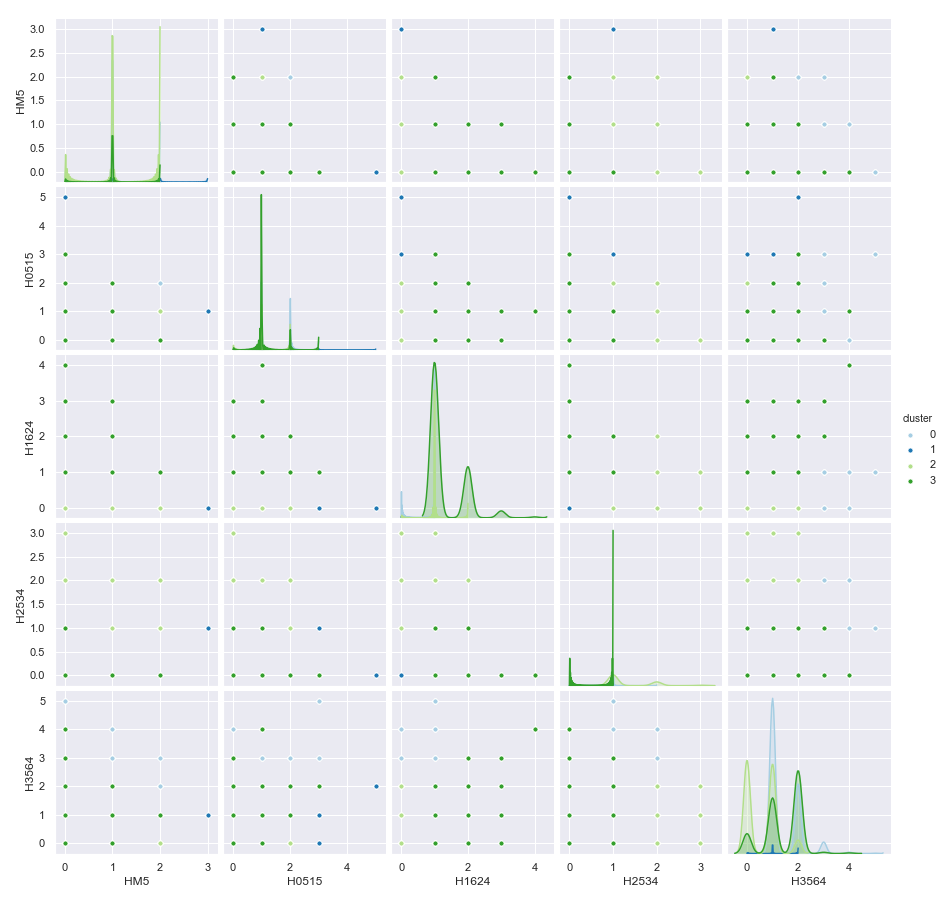
\includegraphics[width=0.9\textwidth]{./imagenes/caso1/scatterMatrix_caso1_K-means}
		\caption{Scatter Matrix usando K-means en el caso de estudio 1.} \label{fig:1}
	\end{figure}
	%------------------------------------------------------------------------
	Para generar la figura 2.2 se ha usado el siguiente fragmento de código (HeatMap): \\

	\lstset{language=python}
	\begin{lstlisting}[frame=single]
def makeHeatmap(data,displayOutput=True,outputName=None):
	meanDF, stdDF = createMeanClusterDF(dataFrame=data)
	meanDF = createNormalizedDF(dataFrame=meanDF)
	anotations = True
	sns.heatmap(data=meanDF, linewidths=.1, cmap='Blues_r', annot=anotations, xticklabels='auto')
	plt.xticks(rotation=0)

	if displayOutput:
		plt.show()

	if outputName != None:
		outputName += '.png'
		print(outputName)
		plt.savefig(outputName)
		plt.clf()
	\end{lstlisting}

	La figura 2.2 representa la media normalizada de los datos totales de cada variable asociados
	a cada cluster usando el algoritmo k-means para el caso 1. (HeatMap) \\

	\begin{figure}[htb]
		\centering
		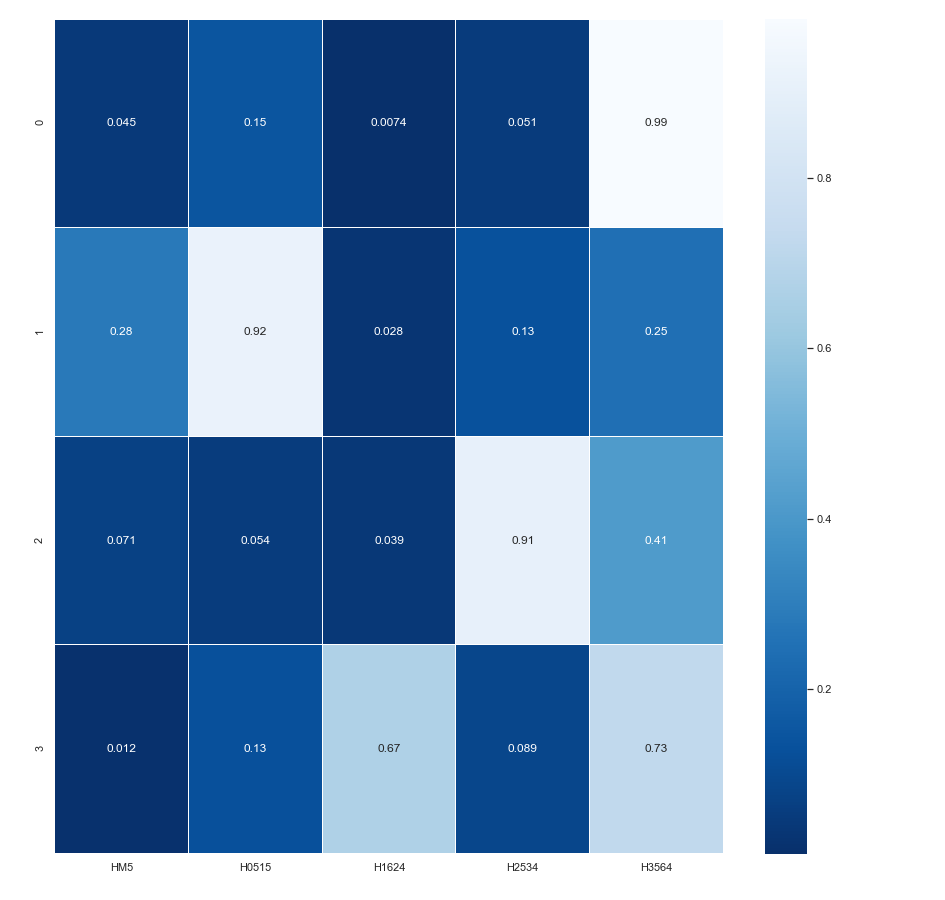
\includegraphics[width=0.9\textwidth]{./imagenes/caso1/heatmap_caso1_K-means}
		\caption{HeatMap usando K-means en el caso de estudio 1.} \label{fig:1}
	\end{figure}

	Para obtener los valores promedios de todas las variables sobre cada cluster, así como sus 
	desviaciones típicas se utiliza el siguiente código: \\

	\lstset{language=python}
	\begin{lstlisting}[frame=single]
def calculateMeanDictionary(cluster,cluster_col = 'cluster'):
	vars = list(cluster)
	vars.remove(cluster_col)
	return dict(np.mean(cluster[vars],axis=0))

def calculateDeviationDictionary(cluster, cluster_col = 'cluster'):
	vars = list(cluster)
	vars.remove(cluster_col)
	return dict(np.std(cluster[vars],axis=0))

def createMeanClusterDF(dataFrame, clusterCol = 'cluster'):
	n_clusters = list(set(dataFrame[clusterCol]))

	my_mean_df = pd.DataFrame()
	my_deviation_df = pd.DataFrame()

	for cluster_n in n_clusters:
		my_cluster = dataFrame[dataFrame[clusterCol] == cluster_n]
		meanDic = calculateMeanDictionary(cluster=my_cluster,cluster_col = clusterCol)
		deviationDic = calculateDeviationDictionary(cluster=my_cluster, cluster_col = clusterCol)
		stdDF = pd.DataFrame(deviationDic, index=[str(cluster_n)])
		auxDF = pd.DataFrame(meanDic,index=[str(cluster_n)])
		my_mean_df = pd.concat([my_mean_df,auxDF])
		my_deviation_df = pd.concat([my_deviation_df,stdDF])

	return [my_mean_df, my_deviation_df]
	\end{lstlisting}

	%------------------------------------------------------------------------
	Para generar la figura 2.3 se ha usado el siguiente fragmento de código: \\

	\lstset{language=python}
	\begin{lstlisting}[frame=single]
def makeDendograma(data, displayOutput=True,outputName=None):
	meanDF, stdDF = createMeanClusterDF(dataFrame=data)   
	linkage_array = hierarchy.ward(meanDF)
	plt.figure()
	plt.clf()
	hierarchy.dendrogram(linkage_array)
	
	if displayOutput:
		plt.show()

	if outputName != None:
		outputName += '.png'
		print(outputName)
		plt.savefig(outputName)
		plt.clf()	
	\end{lstlisting}

	La figura 2.3 es un dendograma , puede ayudar a decidir el numero de grupos que podrían representar
	mejor la estructura de los datos teniendo en cuenta la forma en la que se van anidando los clusters
	y la medida de similitud a la cual lo hacen. \\

	\begin{figure}[htb]
		\centering
		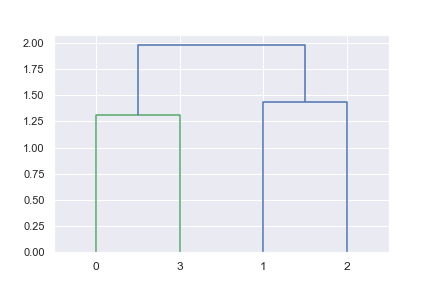
\includegraphics[width=0.6\textwidth]{./imagenes/caso1/dendograma_caso1_K-means}
		\caption{Dendograma usando K-means en el caso de estudio 1.} \label{fig:1}
	\end{figure}

	A continuación se muestra la figura 2.4 , esta es la fusión de las gráficas de 
	Heatmap y de Dendograma.  \\

	\begin{figure}[htb]
		\centering
		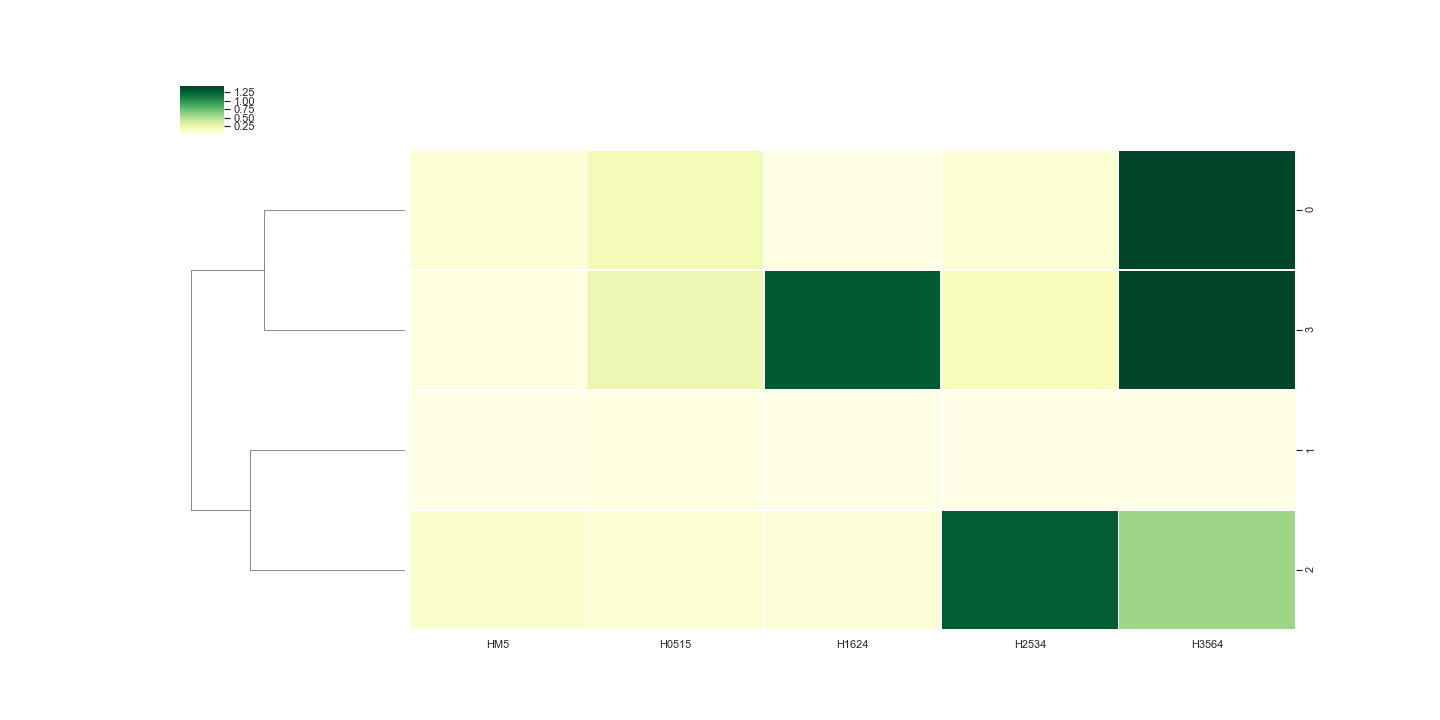
\includegraphics[width=0.9\textwidth]{./imagenes/caso1/heatmapcondendograma_caso1_K-means}
		\caption{HeatMap con Dendograma usando K-means en el caso de estudio 1.} \label{fig:1}
	\end{figure}

	La figura 2.5 esta compuesta por la media de los datos para cada cluster de las variables seleccionadas
	para el estudio. \\ 

	\begin{figure}[htb]
		\centering
		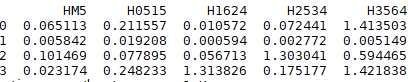
\includegraphics[width=0.6\textwidth]{./imagenes/caso1/medias_datos_caso1_K-means}
		\caption{Medias de los datos seleccionados por cluster K-means.} \label{fig:1}
	\end{figure}


	%----------------------------------------------------------------------
	%							Birch caso 1
	%----------------------------------------------------------------------	

	\subsubsection{Resultados algoritmo Birch caso 1}

	Birch es un algoritmo de aprendizaje no supervisado usado para clustering jerárquico sobre
	grandes cantidades de datos. Una de sus principales ventajas es la capacidad para agrupar 
	incremental y dinámicamente los clusters. En la mayoría de los casos Birch solo necesita un único 
	escaneo de los datos. \\

	%------------------------------------------------------------------------

	La figura 2.6 representa como están distribuidos los diferentes clusters sobre las diferentes variables estudiadas. (ScatterMatrix)\\

	\begin{figure}[htb]
		\centering
		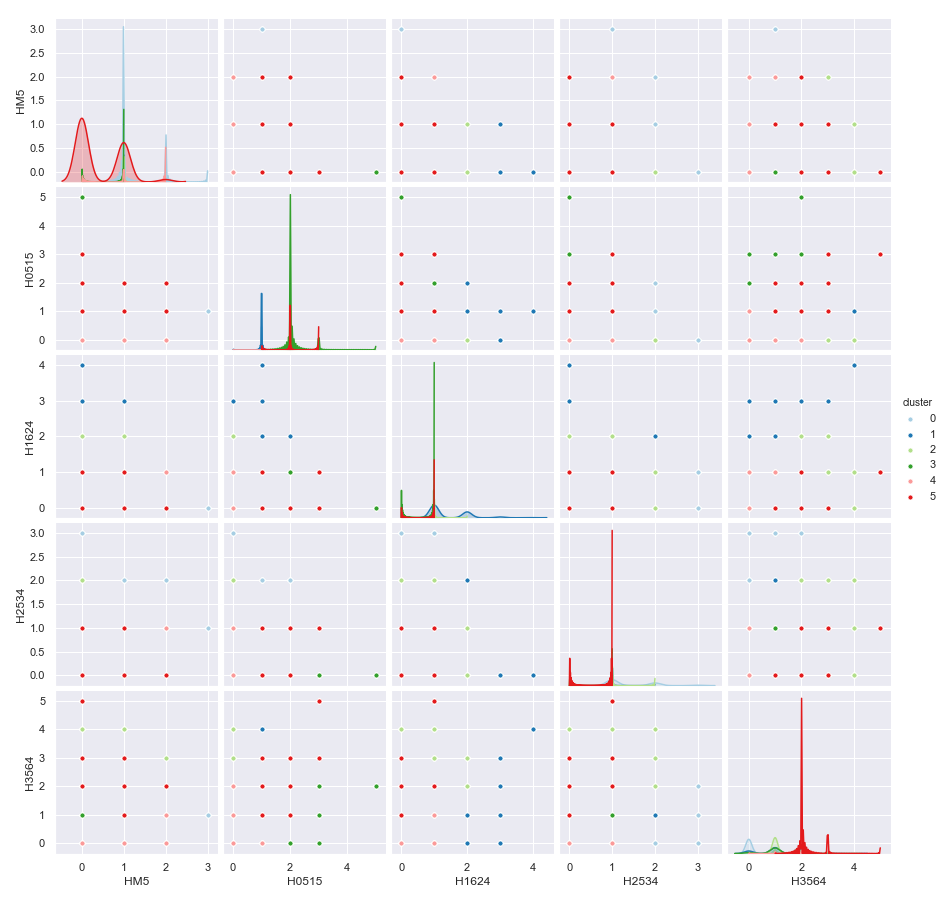
\includegraphics[width=0.9\textwidth]{./imagenes/caso1/scatterMatrix_caso1_Birch}
		\caption{Scatter Matrix usando Birch en el caso de estudio 1.} \label{fig:1}
	\end{figure}
	%------------------------------------------------------------------------

	La figura 2.7 representa la media normalizada de los datos totales de cada variable asociados
	a cada cluster usando el algoritmo Birch para el caso 1. (HeatMap) \\

	\begin{figure}[htb]
		\centering
		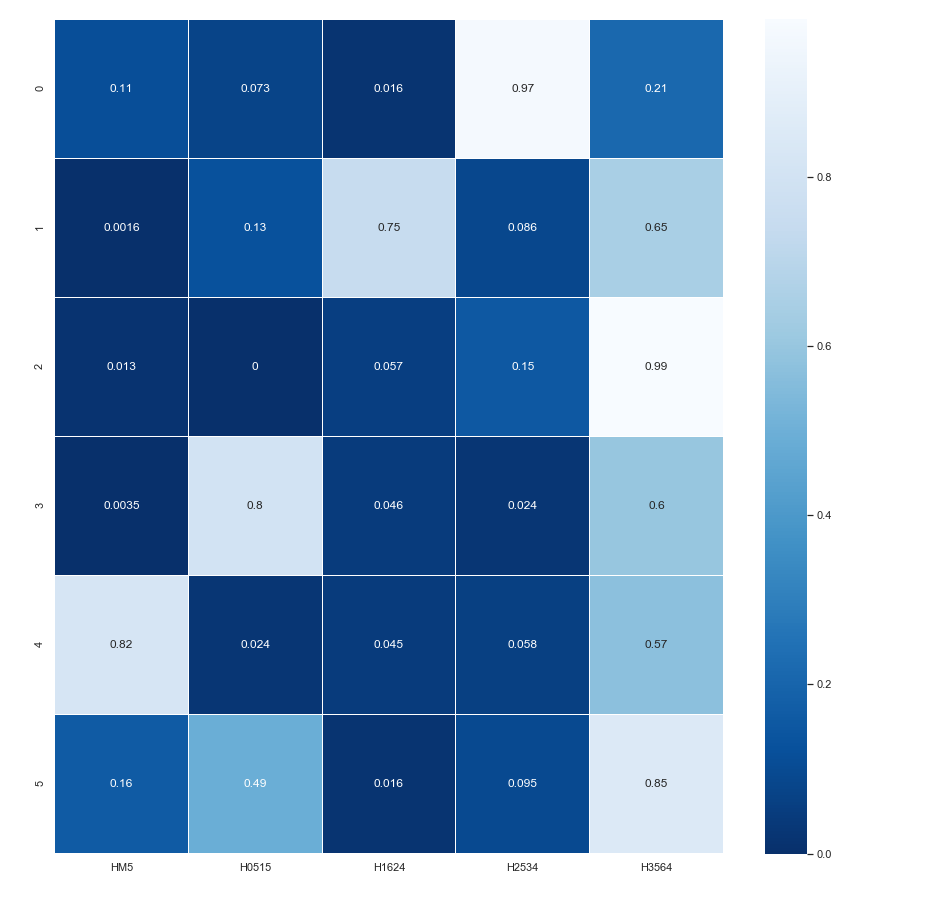
\includegraphics[width=0.9\textwidth]{./imagenes/caso1/heatmap_caso1_Birch}
		\caption{HeatMap usando Birch en el caso de estudio 1.} \label{fig:1}
	\end{figure}

	%------------------------------------------------------------------------

	La figura 2.8 es un dendograma , puede ayudar a decidir el numero de grupos que podrían representar
	mejor la estructura de los datos teniendo en cuenta la forma en la que se van anidando los clusters
	y la medida de similitud a la cual lo hacen. \\

	\begin{figure}[htb]
		\centering
		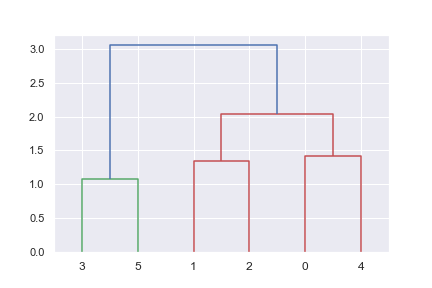
\includegraphics[width=0.6\textwidth]{./imagenes/caso1/dendograma_caso1_Birch}
		\caption{Dendograma usando Birch en el caso de estudio 1.} \label{fig:1}
	\end{figure}

	A continuación se muestra la figura 2.9 , esta es la fusión de las gráficas de 
	Heatmap y de Dendograma.  \\

	\begin{figure}[htb]
		\centering
		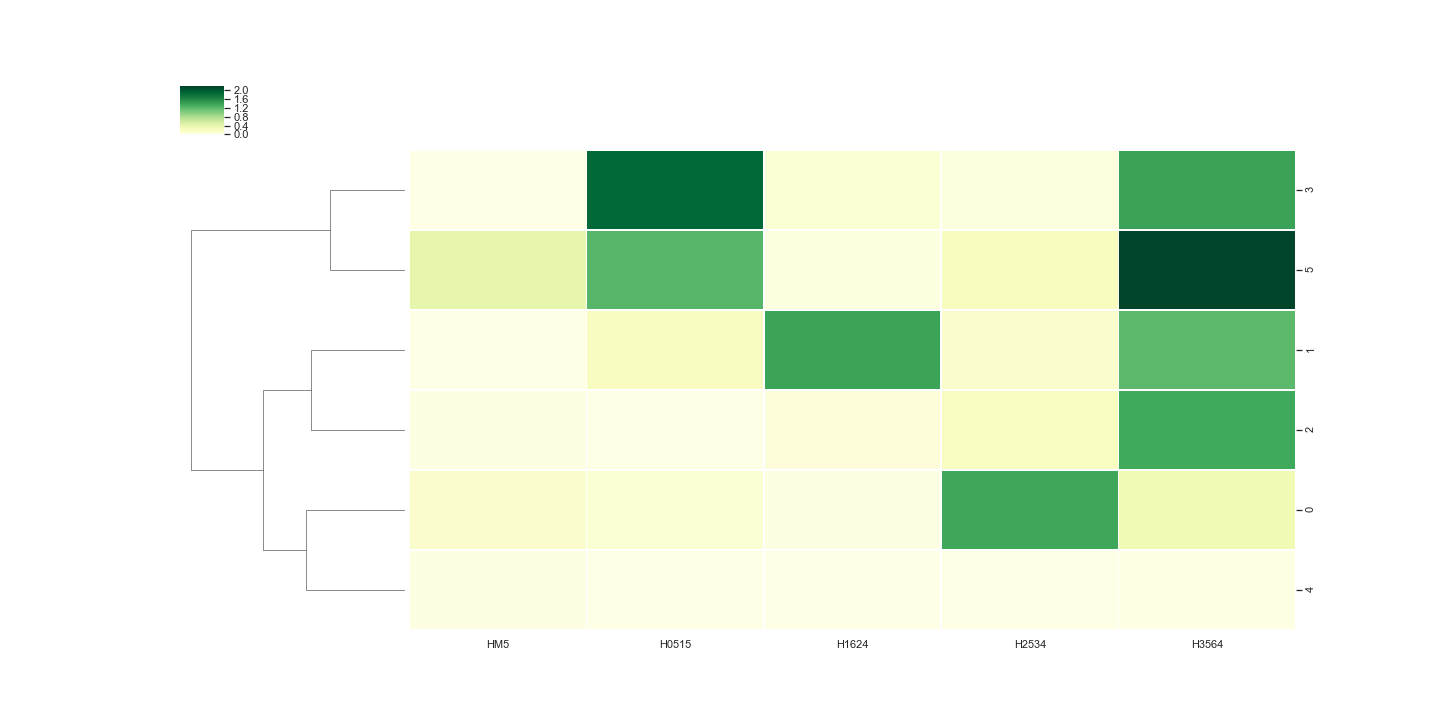
\includegraphics[width=0.9\textwidth]{./imagenes/caso1/heatmapcondendograma_caso1_Birch}
		\caption{HeatMap con Dendograma usando Birch en el caso de estudio 1.} \label{fig:1}
	\end{figure}

	La figura 2.10 esta compuesta por la media de los datos para cada cluster de las variables seleccionadas
	para el estudio. \\ 

	\begin{figure}[htb]
		\centering
		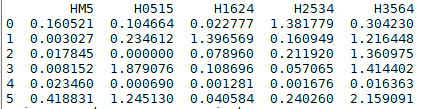
\includegraphics[width=0.6\textwidth]{./imagenes/caso1/medias_datos_caso1_Birch}
		\caption{Medias de los datos seleccionados por cluster Birch.} \label{fig:1}
	\end{figure}

	%----------------------------------------------------------------------
	%							Ward caso 1
	%----------------------------------------------------------------------	

	\subsubsection{Resultados algoritmo Ward caso 1}

	El método de Ward es un procedimiento jerárquico en el cual, en cada etapa, 
	se unen los dos clusters para los cuales se tenga el menor incremento en el valor 
	total de la suma de los cuadrados de las diferencias,
	dentro de cada cluster, de cada individuo al centroide del cluster. \\

	%------------------------------------------------------------------------

	La figura 2.11 representa como están distribuidos los diferentes clusters sobre las diferentes variables estudiadas. (ScatterMatrix)\\

	\begin{figure}[htb]
		\centering
		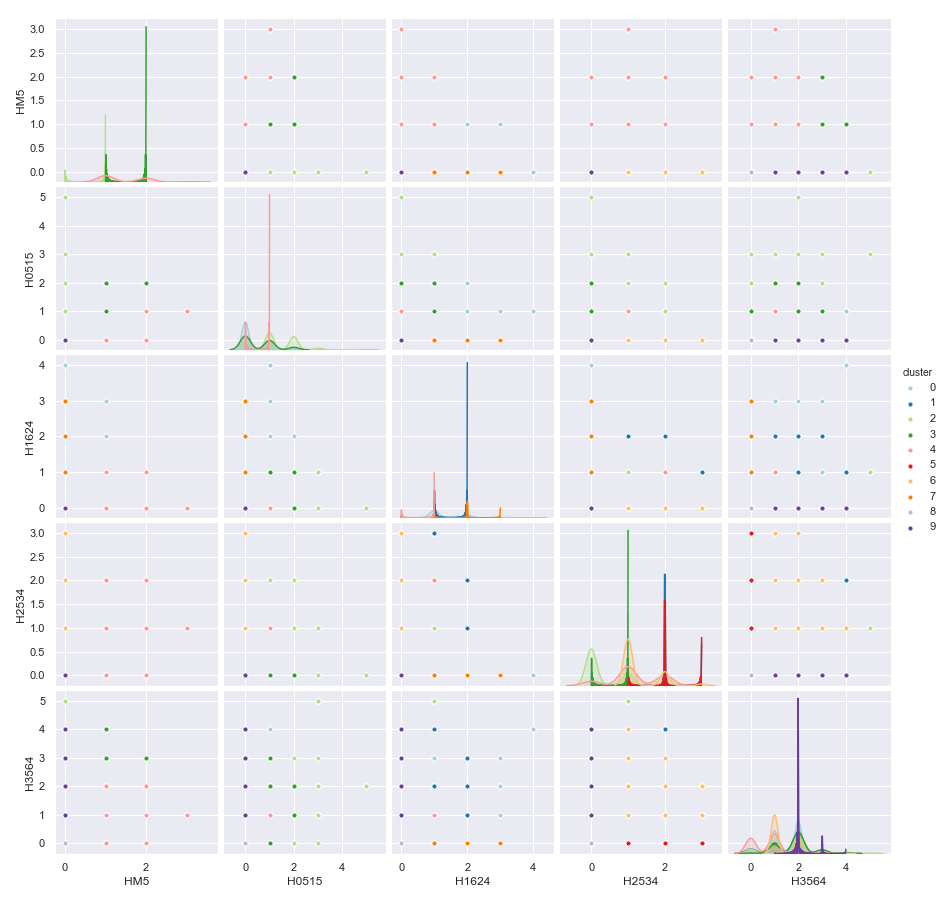
\includegraphics[width=0.9\textwidth]{./imagenes/caso1/scatterMatrix_caso1_Ward}
		\caption{Scatter Matrix usando Ward en el caso de estudio 1.} \label{fig:1}
	\end{figure}
	%------------------------------------------------------------------------

	La figura 2.12 representa la media normalizada de los datos totales de cada variable asociados
	a cada cluster usando el algoritmo Ward para el caso 1. (HeatMap) \\

	\begin{figure}[htb]
		\centering
		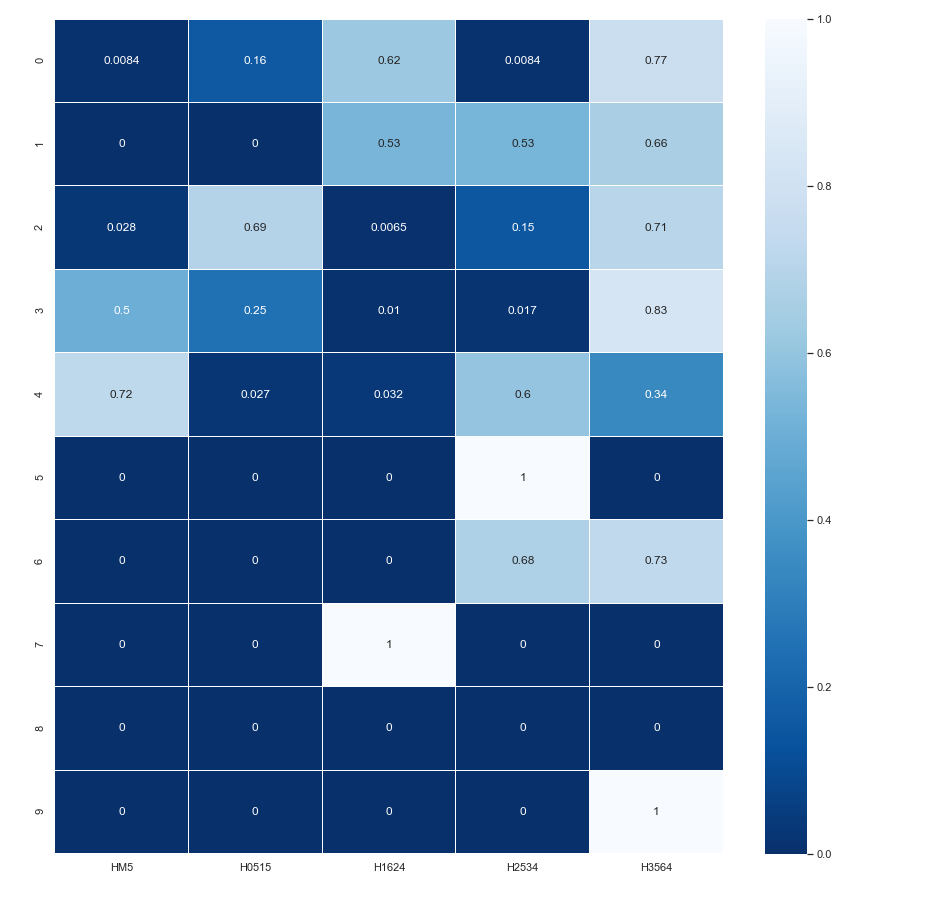
\includegraphics[width=0.9\textwidth]{./imagenes/caso1/heatmap_caso1_Ward}
		\caption{HeatMap usando Ward en el caso de estudio 1.} \label{fig:1}
	\end{figure}

	%------------------------------------------------------------------------

	La figura 2.13 es un dendograma , puede ayudar a decidir el numero de grupos que podrían representar
	mejor la estructura de los datos teniendo en cuenta la forma en la que se van anidando los clusters
	y la medida de similitud a la cual lo hacen. \\

	\begin{figure}[htb]
		\centering
		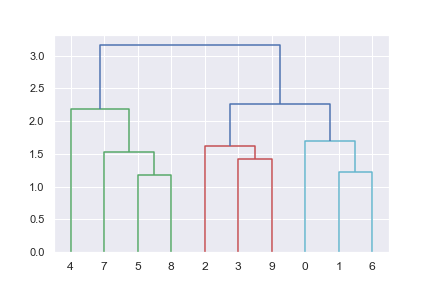
\includegraphics[width=0.6\textwidth]{./imagenes/caso1/dendograma_caso1_Ward}
		\caption{Dendograma usando Ward en el caso de estudio 1.} \label{fig:1}
	\end{figure}

	A continuación se muestra la figura 2.14 , esta es la fusión de las gráficas de 
	Heatmap y de Dendograma.  \\

	\begin{figure}[htb]
		\centering
		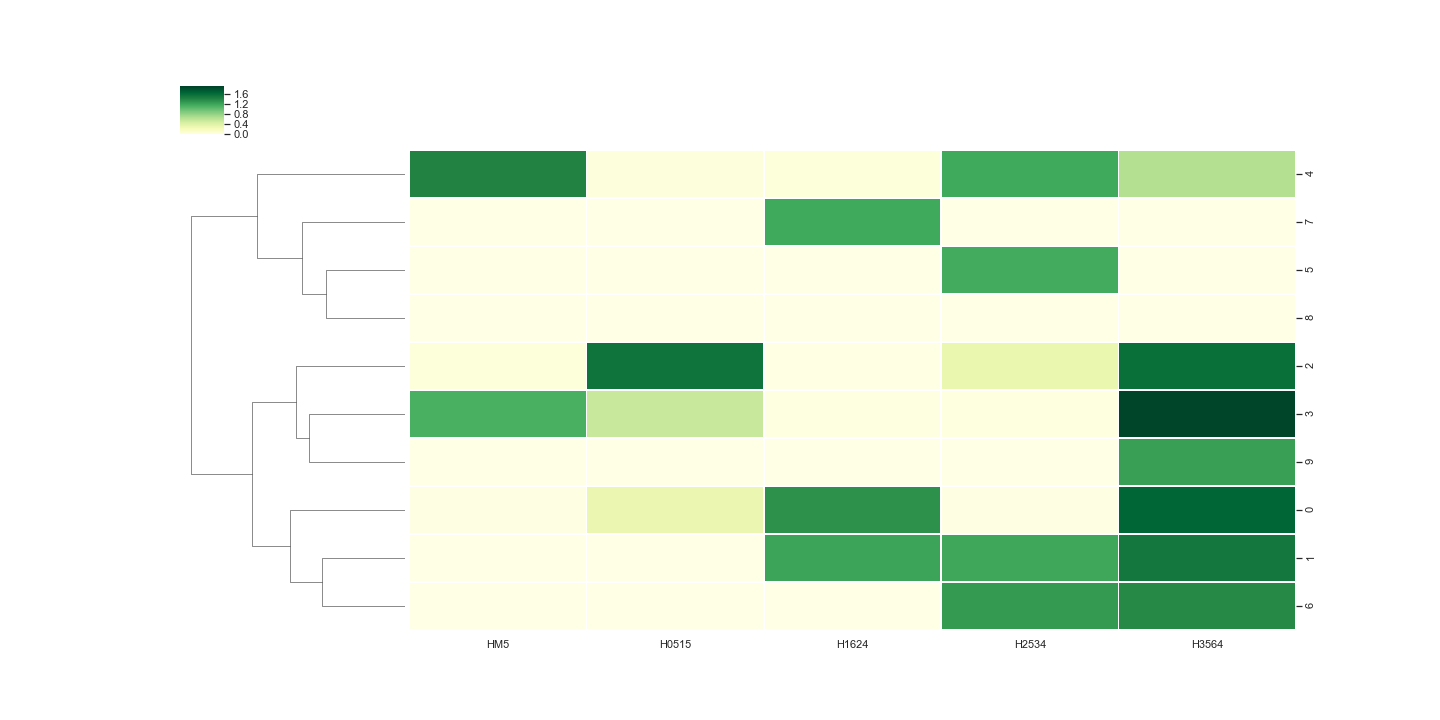
\includegraphics[width=0.9\textwidth]{./imagenes/caso1/heatmapcondendograma_caso1_Ward}
		\caption{HeatMap con Dendograma usando Ward en el caso de estudio 1.} \label{fig:1}
	\end{figure}

	La figura 2.15 esta compuesta por la media de los datos para cada cluster de las variables seleccionadas
	para el estudio. \\ 

	\begin{figure}[htb]
		\centering
		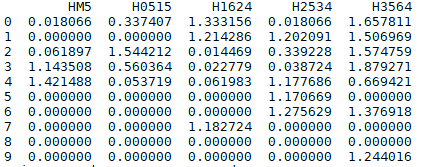
\includegraphics[width=0.6\textwidth]{./imagenes/caso1/medias_datos_caso1_Ward}
		\caption{Medias de los datos seleccionados por cluster Ward.} \label{fig:1}
	\end{figure}

	%----------------------------------------------------------------------
	%							MeanShift caso 1
	%----------------------------------------------------------------------	

	\subsubsection{Resultados algoritmo MeanShift caso 1}

	El algoritmo Mean Shift es una técnica de clustering no paramétrica que no requiere conocimiento
	del numero de clusters. Dado N puntos de datos, en un espacio d-dimensional, el núcleo de densidad
	miltivariado se estima obtener con K(x) \cite{cite6} \\

	%------------------------------------------------------------------------

	La figura 2.16 representa como están distribuidos los diferentes clusters sobre las diferentes variables estudiadas. (ScatterMatrix)\\

	\begin{figure}[htb]
		\centering
		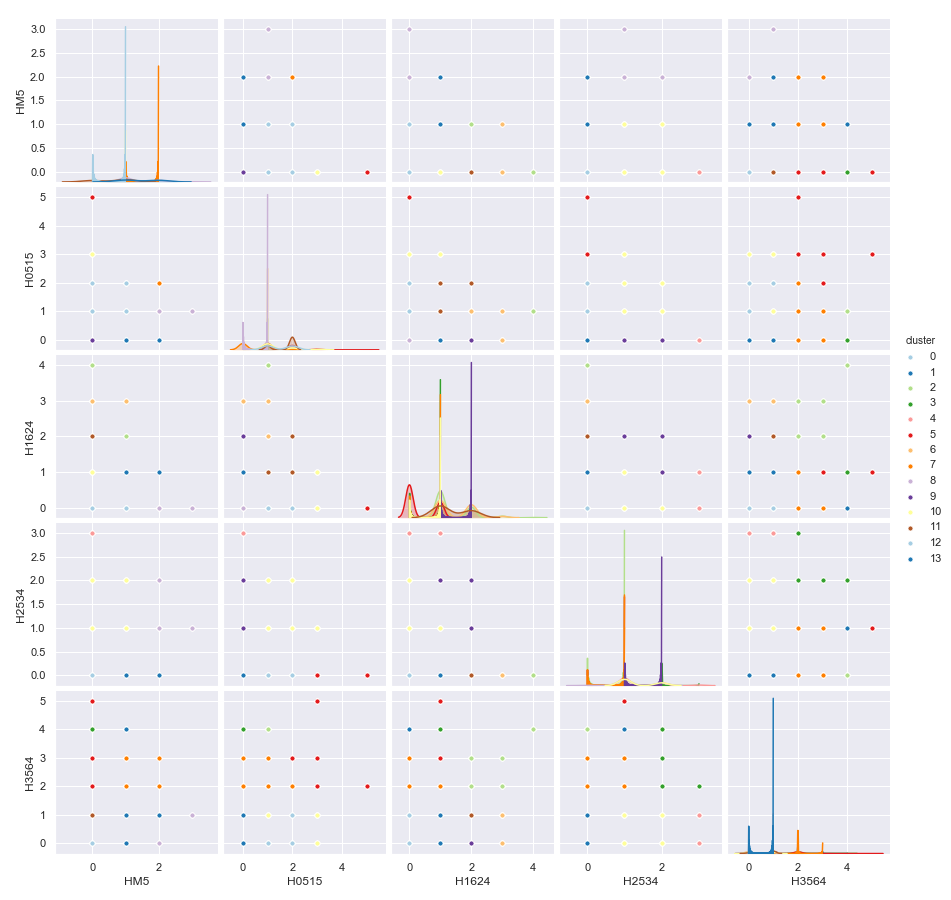
\includegraphics[width=0.9\textwidth]{./imagenes/caso1/scatterMatrix_caso1_MeanShift}
		\caption{Scatter Matrix usando MeanShift en el caso de estudio 1.} \label{fig:1}
	\end{figure}
	%------------------------------------------------------------------------

	La figura 2.17 representa la media normalizada de los datos totales de cada variable asociados
	a cada cluster usando el algoritmo MeanShift para el caso 1. (HeatMap) \\

	\begin{figure}[htb]
		\centering
		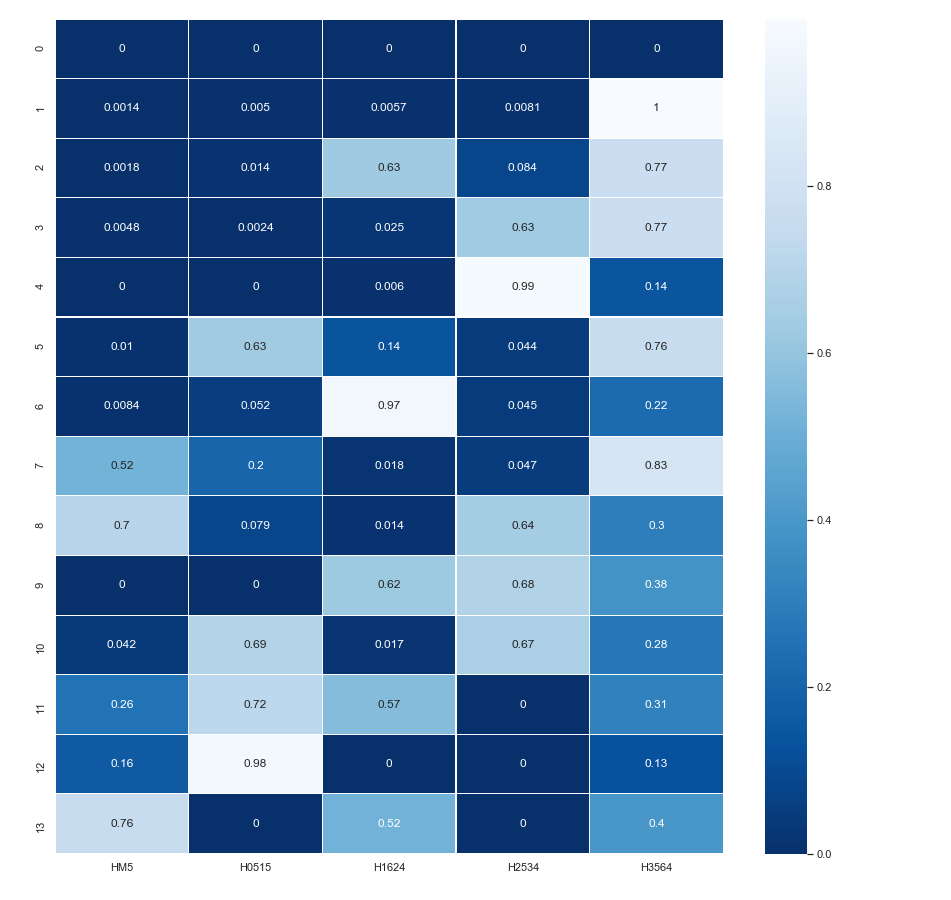
\includegraphics[width=0.9\textwidth]{./imagenes/caso1/heatmap_caso1_MeanShift}
		\caption{HeatMap usando MeanShift en el caso de estudio 1.} \label{fig:1}
	\end{figure}

	%------------------------------------------------------------------------

	La figura 2.18 es un dendograma , puede ayudar a decidir el numero de grupos que podrían representar
	mejor la estructura de los datos teniendo en cuenta la forma en la que se van anidando los clusters
	y la medida de similitud a la cual lo hacen. \\

	\begin{figure}[htb]
		\centering
		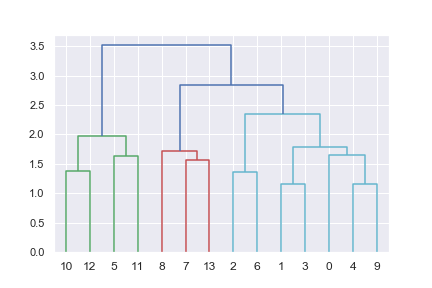
\includegraphics[width=0.6\textwidth]{./imagenes/caso1/dendograma_caso1_MeanShift}
		\caption{Dendograma usando MeanShift en el caso de estudio 1.} \label{fig:1}
	\end{figure}

	A continuación se muestra la figura 2.19 , esta es la fusión de las gráficas de 
	Heatmap y de Dendograma.  \\

	\begin{figure}[htb]
		\centering
		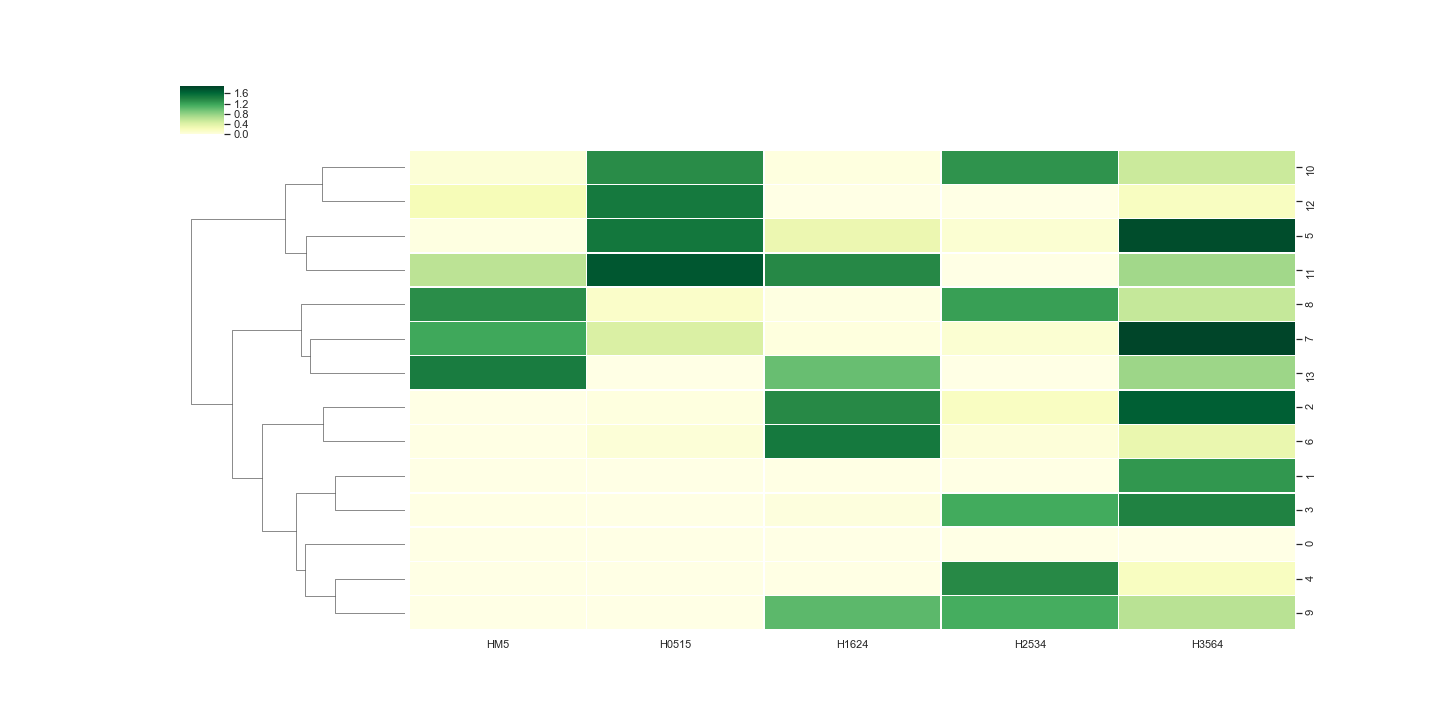
\includegraphics[width=0.9\textwidth]{./imagenes/caso1/heatmapcondendograma_caso1_MeanShift}
		\caption{HeatMap con Dendograma usando MeanShift en el caso de estudio 1.} \label{fig:1}
	\end{figure}

	La figura 2.20 esta compuesta por la media de los datos para cada cluster de las variables seleccionadas
	para el estudio. \\ 

	\begin{figure}[htb]
		\centering
		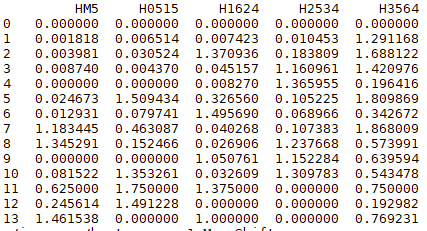
\includegraphics[width=0.6\textwidth]{./imagenes/caso1/medias_datos_caso1_MeanShift}
		\caption{Medias de los datos seleccionados por cluster MeanShift.} \label{fig:1}
	\end{figure}

	%----------------------------------------------------------------------
	%							spectral caso 1
	%----------------------------------------------------------------------	

	\subsubsection{Resultados algoritmo Spectral caso 1}

	las técnicas de agrupamiento espectral hacen uso del espectro (valores propios)
	de la matriz [similitud] de los datos para realizar reducción de dimensionalidad 
	antes de la agrupación en un menor número de dimensiones. La matriz de similitud se 
	proporciona como una entrada y consta de una evaluación cuantitativa de la similitud 
	relativa de cada par de puntos en el conjunto de datos. \cite{cite5} \\

	%------------------------------------------------------------------------

	La figura 2.21 representa como están distribuidos los diferentes clusters sobre las diferentes variables estudiadas. (Scatter Matrix)\\

	\begin{figure}[htb]
		\centering
		\includegraphics[width=0.9\textwidth]{./imagenes/caso1/scatterMatrix_caso1_spectral}
		\caption{Scatter Matrix usando spectral en el caso de estudio 1.} \label{fig:1}
	\end{figure}
	%------------------------------------------------------------------------

	La figura 2.22 representa la media normalizada de los datos totales de cada variable asociados
	a cada cluster usando el algoritmo spectral para el caso 1. (HeatMap) \\

	\begin{figure}[htb]
		\centering
		\includegraphics[width=0.9\textwidth]{./imagenes/caso1/heatmap_caso1_spectral}
		\caption{HeatMap usando spectral en el caso de estudio 1.} \label{fig:1}
	\end{figure}

	%------------------------------------------------------------------------

	La figura 2.23 es un dendograma , puede ayudar a decidir el numero de grupos que podrían representar
	mejor la estructura de los datos teniendo en cuenta la forma en la que se van anidando los clusters
	y la medida de similitud a la cual lo hacen. \\

	\begin{figure}[htb]
		\centering
		\includegraphics[width=0.6\textwidth]{./imagenes/caso1/dendograma_caso1_spectral}
		\caption{Dendograma usando spectral en el caso de estudio 1.} \label{fig:1}
	\end{figure}

	A continuación se muestra la figura 2.24 , esta es la fusión de las gráficas de 
	Heatmap y de Dendograma.  \\

	\begin{figure}[htb]
		\centering
		\includegraphics[width=0.9\textwidth]{./imagenes/caso1/heatmapcondendograma_caso1_spectral}
		\caption{HeatMap con Dendograma usando spectral en el caso de estudio 1.} \label{fig:1}
	\end{figure}

	La figura 2.25 esta compuesta por la media de los datos para cada cluster de las variables seleccionadas
	para el estudio. \\ 

	\begin{figure}[htb]
		\centering
		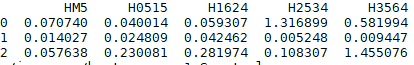
\includegraphics[width=0.6\textwidth]{./imagenes/caso1/medias_datos_caso1_spectral}
		\caption{Medias de los datos seleccionados por cluster spectral.} \label{fig:1}
	\end{figure}

	%----------------------------------------------------------------------
	%						Algoritmos Modificados Caso 1
	%----------------------------------------------------------------------

	\subsubsection[Algoritmos modificados en el caso 1]{Algoritmos modificados en el caso 1}

	En esta sección se va a exponer la modificación de los parámetros de dos algoritmos distintos y para ver sus diferencias
	se van a comparar los resultados de las métricas obtenidas en las secciones previas. \\

	El primer algoritmo que vamos a modificar por su pésima métrica de CH es Birch , intentando 
	aumentar su valor disminuido el numero de clusters a 4 y el segundo algoritmo que vamos a modificar es Ward, y vamos a incrementar su numero de clusters a 35
	para ver que resultados obtenemos y compararlos con la anterior ejecución. \\

	La figura 2.26 muestra la antigua tabla pero ahora con las métricas de la ejecución de estos dos algoritmos modificados.
	En ella se aprecia que las modificaciones de los parámetros han sido exitosas en el caso de Ward
	y fatales en el caso del algoritmo Birch. En el algoritmo Birch modificado se han disminuido bastante la métrica CH y la métrica SH 
	.En el algoritmo Ward modificado se han incrementado muchísimo las métricas
	CH Y SH al aumentar el numero de clusters. Por lo que podemos predecir que aumentando el numero de clusters del resto de
	algoritmo se obtendrían mejores resultados. 

	\begin{figure}[htb]
		\centering
		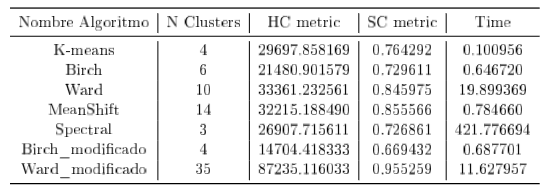
\includegraphics[width=0.9\textwidth]{./imagenes/caso1/algoritmos_modificados_caso1}
		\caption{Metricas obtenidas usando algoritmos modificados en el caso de estudio 1.} \label{fig:1}
	\end{figure}

	%--------------------------- Birch -----------------------------------
	\subsubsection{Algoritmo modificado Birch caso 1}

	La figura 2.27 representa como están distribuidos los diferentes clusters sobre las diferentes variables con el 
	algoritmo Birch. (ScatterMatrix)\\

	\begin{figure}[htb]
		\centering
		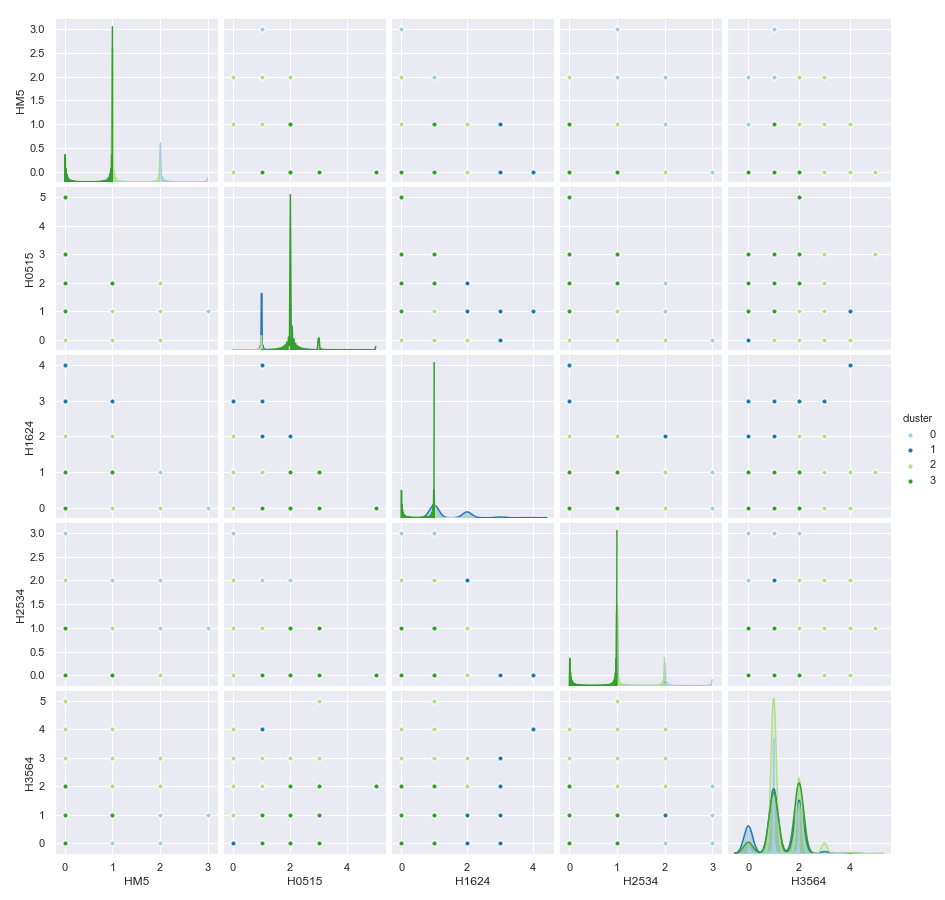
\includegraphics[width=0.9\textwidth]{./imagenes/caso1/scatterMatrix_caso1_Birch_modificado}
		\caption{Scatter Matrix usando Birch modificado en el caso de estudio 1.} \label{fig:1}
	\end{figure}
	
	A continuación se muestra la figura 2.28 , esta es la fusión de las gráficas de 
	Heatmap y de Dendograma con el algoritmo Birch modificado.  \\

	\begin{figure}[htb]
		\centering
		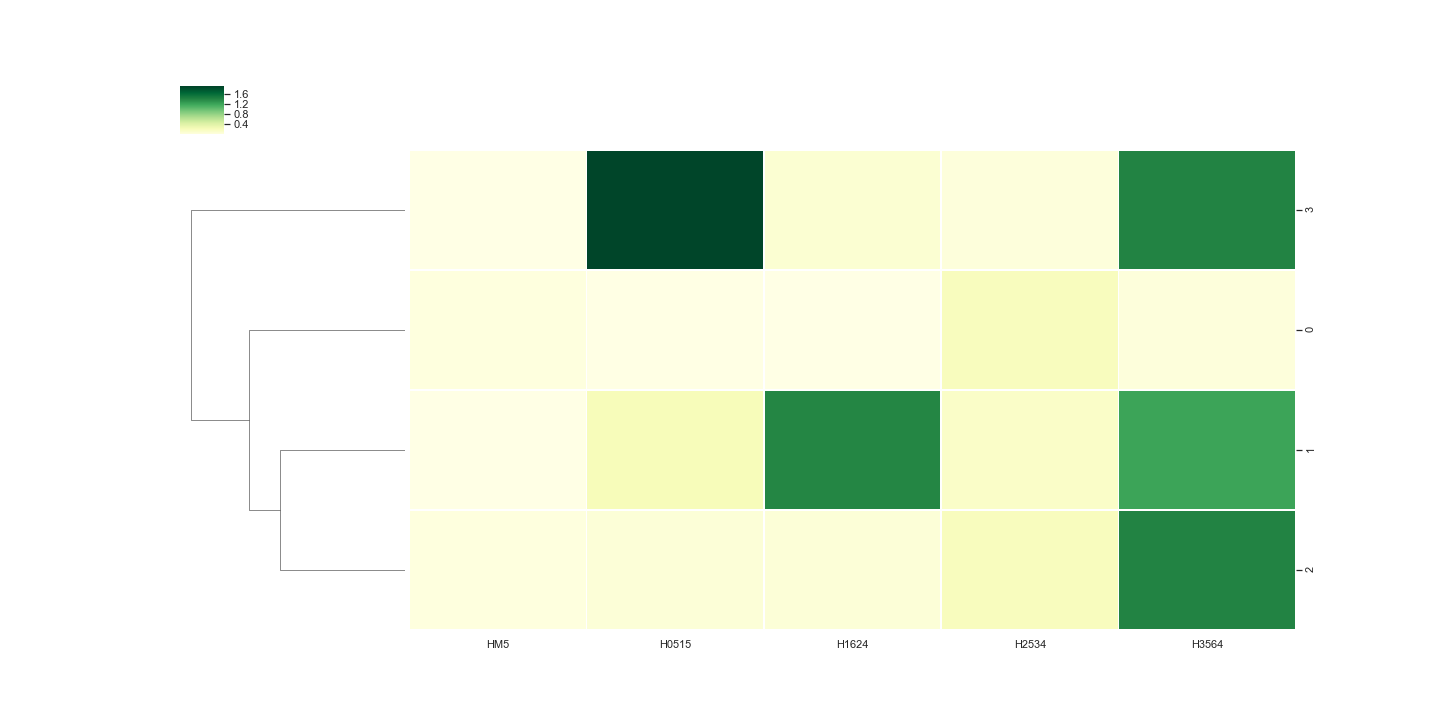
\includegraphics[width=0.9\textwidth]{./imagenes/caso1/heatmapcondendograma_caso1_Birch_modificado}
		\caption{HeatMap con Dendograma usando Birch modificado en el caso de estudio 1.} \label{fig:1}
	\end{figure}

	%--------------------------- Ward -----------------------------------
	\subsubsection{Algoritmo modificado Ward caso 1}

	La figura 2.29 representa como están distribuidos los diferentes clusters sobre las diferentes variables con el 
	algoritmo Ward. (ScatterMatrix)\\

	\begin{figure}[htb]
		\centering
		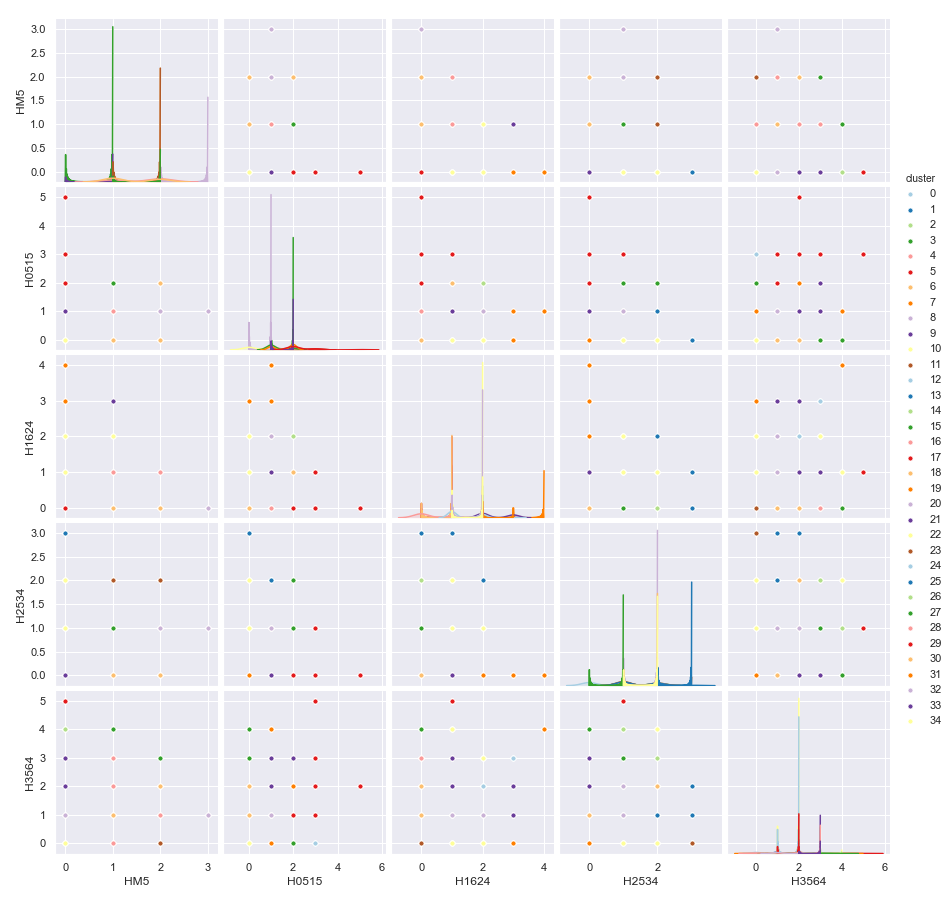
\includegraphics[width=0.9\textwidth]{./imagenes/caso1/scatterMatrix_caso1_Ward_modificado}
		\caption{Scatter Matrix usando Ward modificado en el caso de estudio 1.} \label{fig:1}
	\end{figure}
	
	A continuación se muestra la figura 2.30 , esta es la fusión de las gráficas de 
	Heatmap y de Dendograma con el algoritmo Ward modificado.  \\

	\begin{figure}[htb]
		\centering
		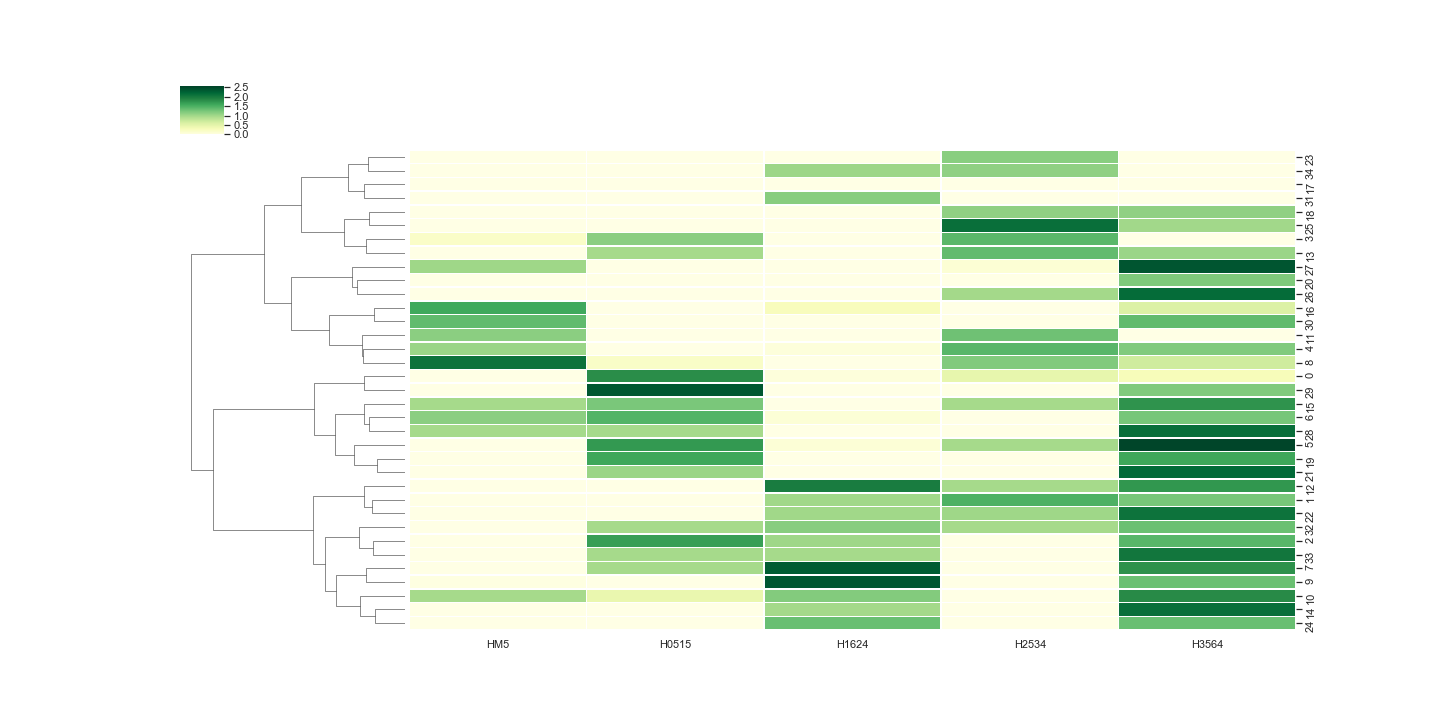
\includegraphics[width=0.9\textwidth]{./imagenes/caso1/heatmapcondendograma_caso1_Ward_modificado}
		\caption{HeatMap con Dendograma usando Ward modificado en el caso de estudio 1.} \label{fig:1}
	\end{figure}

	%----------------------------------------------------------------------
	%					Interpretacion de la segmentacion
	%----------------------------------------------------------------------

	\subsubsection[Interpretacion de la segmentacion caso 1]{Interpretacion de la segmentacion caso 1}

	Para terminar con el estudio de este caso , vamos a interpretar las visualizaciones producidas
	por las ejecuciones de los algoritmos, recalcando de que los datos obtenidos son los de las personas con uno o mas
	miembros mayores de 64 años en sus familias, incluyéndose a estas. \\

	%----------------------------------------------------------------------
	Para el algoritmo K-Means podemos apreciar que en el cluster cero se agrupan aquellas 
	familias con dos o mas miembros entre 35 y 64 , con 3 miembros o menos entre 5 y 15 años y en algunos casos con miembros entre
	16 y 24 o menores de 15. En el cluster uno se agrupan aquellas familias con 3 miembros o mas entre 5 y 15 años , con 
	tres miembros menores de 5 años , y uno o dos miembros entre 35 y 64 años. Puntualmente también hay miembros entre 
	16 y 34 años. En el cluster dos se agrupan aquellas familias con dos miembros entre 25 y 34 y varios miembros menores de 15 años y ningun miembro
	en el rango 35-64, por lo que podríamos decir que son parejas de jóvenes (24-34) que viven con sus padres y con sus hijos. 
	En el cluster 3 se agrupan aquellas familias con algún miembro entre 0 y 15 , un miembro entre 16 y 34 años y 
	con entre cero y dos miembros entre 35 y 64. \\
	%----------------------------------------------------------------------
	Para el algoritmo Birch podemos apreciar que se asemeja bastante al caso anterior de 
	K-means , pero ahora con un cluster mas. En el cluster cero se agrupan aquellas familias con varios miembros entre 
	25 y 34 años y varios miembros menores de 5 años. En el cluster uno se agrupan aquellas familias con varios miembros 
	entre 35 y 64 y varios miembros entre 16 y 24. En el cluster dos se agrupan aquellas familias con varios miembros entre
	35 y 64 y algun miembro entre 25 y 34. En el cluster tres se agrupan aquellas familias varios miembros entre cinco
	y 15 años y varios miembros entre 35 y 64. En el cluster cuatro tenemos agrupadas a aquellas familias con varios miembros
	entre 35 y 64 y algun miembro menor de 15 años. En el quinto cluster tenemos aquellas familias con al menos dos menores
	de cinco años , un miembro entre 25 y 34 y de dos a cuatro miembros entre 35 y 64 , por lo que podríamos decir que en este tipo
	de familias viven personas de entre todos los rangos de edades.  \\
	%----------------------------------------------------------------------
	Para el algoritmo Ward también se pueden apreciar similitudes respecto a los algoritmos comentados anteriormente , pero
	en este caso tenemos los datos agrupados en 9 clusters . En los clusters de 0 al 4 se han agrupado los datos de forma
	similar a los algoritmos anteriores, pero en los clusters del quinto al noveno presenciamos un agrupamiento distinto.
	En el cluster 5 se han agrupado aquellas familias solo con miembros entre 25 y 34 . En el cluster 6 se han agrupado aquellas
	familias con miembro solo entre 25 y 64. En el cluster 7 se han agrupado aquellas familias solo con miembros entre 16 y 24.
	En el cluster 8 se han agrupado aquellas personas que son mayores de 64 años. Y por ultimo en el cluster 9 se han 
	agrupado aquellas familias con solo miembros (entre dos y 4) entre 35 y 64 años. Posiblemente familias de hermanos que vivan junto
	a sus padres. \\
	%----------------------------------------------------------------------
	Para el algoritmo Spectral, se puede apreciar que comparado con el resto de algoritmos 
	los agrupamientos han sido muy heterogéneos , debido a la falta de numero de clusters. En el cluster cero se han agrupado 
	principalmente aquellas familias con varios miembros entre 25 y 34 años. En el cluster uno se han agrupado aquellas 
	familias con varios miembros entre 16 y 2y. En el cluster numero dos se han agrupado aquellas familias con varios miembros
	entre 35 y 64 .
	%----------------------------------------------------------------------
	Para el caso del algoritmo Ward modificado , al aumentar el numero de clusters permitimos la segmentación en un mayor numero 
	de grupos , pudiendo así segmentar mejor a los diferentes tipos de familias. Se puede apreciar que en el cluster 17 se agrupan 
	aquellas personas mayores que viven solas. Así como que en el cluster 32 se agrupan aquellas familias con miembros prácticamente
	en todos los rangos de edades. \\

	%----------------------------------------------------------------------
	%							Caso de estudio 2
	%----------------------------------------------------------------------	
	
	\subsection[Caso de estudio 2. Personas solteras que no vivan con personas mayores de 65 ni menores de 15.]{Segundo caso de estudio: Personas solteras que no vivan con personas mayores de 65 ni menores de 15.}

	En este segundo caso de estudio nos vamos a centrar en personas que no viven en su hogar con personas mayores de 65 ni menores de 15 años, 
	analizaremos la edad de estas personas y el numero de personas y rango de edades dentro del hogar .
	Las variables que vamos a utilizar son : \\

	EDAD  : Edad de la persona  \\   
	TAMNUC : Tamaño del núcleo \\
	H1624 : Número de personas de 16 a 24 años en el hogar  \\
	H2534  : Número de personas de 25 a 34 años en el hogar \\
	H3564 : Número de personas de 35 a 64 años en el hogar   \\

	En la figura 2.31 se muestran los datos asociados a cada algoritmo usado para este caso de estudio
	de personas que viven con personas mayores , datos como el numero de clusters que se han usado,
	la métrica Calinski-harabasz (CH) , la métrica Siljouette (SC) y el tiempo en segundos que ha tardado
	el algoritmo para ejecutarse . Para este caso de estudio se han contado con un total de 22628 instancias.\\

	\begin{figure}[htb]
		\centering
		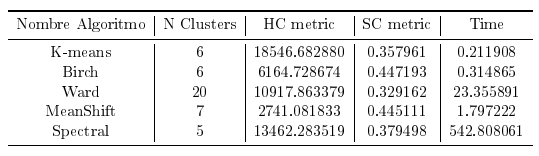
\includegraphics[width=0.9\textwidth]{./imagenes/caso2/metricas_algoritmos_caso2}
		\caption{Resultados y caracteristicas de los algoritmos para el caso de estudio 2.} \label{fig:1}
	\end{figure}

	En este caso , vemos como para el indice Calinski-Harabasz hay un algoritmo que esta claramente 
	en cabeza, K-means. Por detrás esta el algoritmo Spectal , y le sigue el algoritmo Ward. Por ultimo 
	tenemos los pésimos resultados de los algoritmos Birch y MeanShift.  \\

	Para el indice Silhouette no ocurre lo mismo que para el Calinski-Harabasz, ya que todos los resultados se encuentra a la par,
	teniendo MeanShift y Birch las mejores métricas en este caso. \\
	
	Quedando los algoritmos K-means y Spectral como los que mejores se comportan podríamos clonar el numero de clusters usados en ese algoritmo 
	para ver si se producen mejoras en las métricas de los demás algoritmos.\\

	Por ultimo cabe decir que el algoritmo Spectral es que mayor tiempo de ejecución tiene. En las siguientes subsecciones
	se muestran gráficas y tablas de algoritmos asociadas a cada algoritmo usado para cada caso de estudio
	, y al final exponemos un análisis de los resultados obtenidos.\\

	Cabe destacar que se ha realizado la eliminación de aquellos clusters con pocos datos (ouliers) . Se ha realizado mediante un 
	filtrado a los clusters con menos de 5 elementos. \\

	%----------------------------------------------------------------------
	%							k-means caso 2
	%----------------------------------------------------------------------	

	\subsubsection{Resultados algoritmo K-Means caso 2}

	%------------------------------------------------------------------------

	La figura 2.32 representa como están distribuidos los diferentes clusters sobre las diferentes variables estudiadas. (Scatter Matrix)\\

	\begin{figure}[htb]
		\centering
		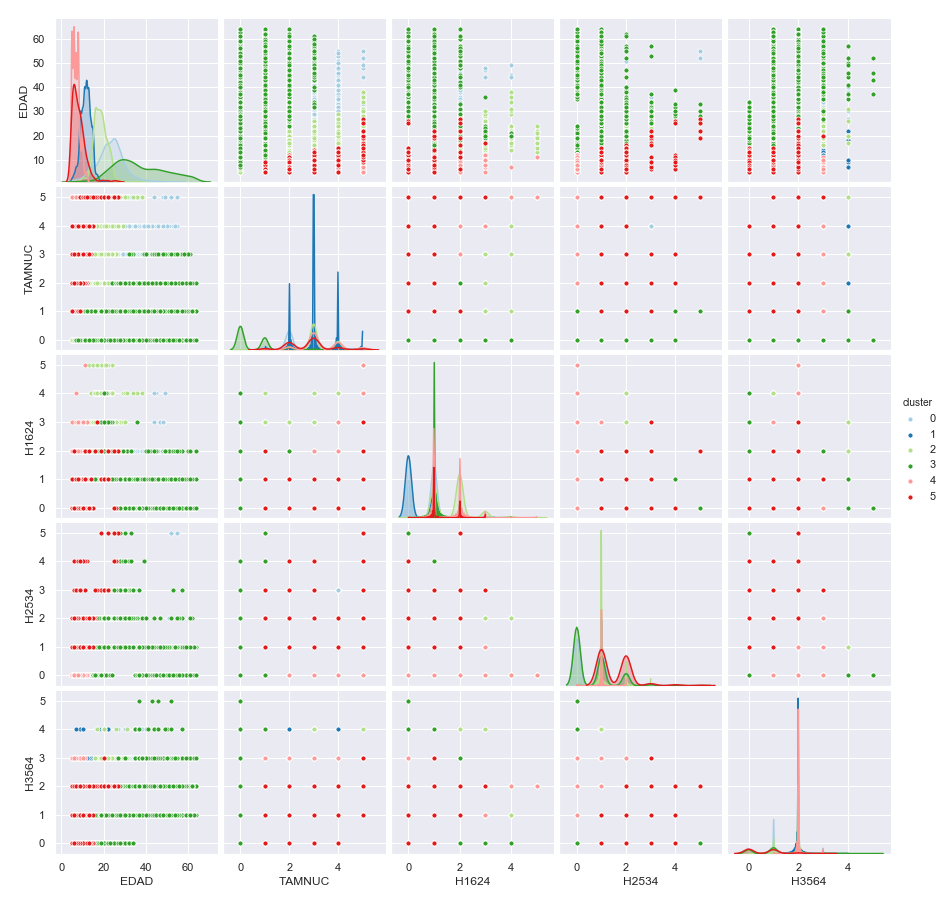
\includegraphics[width=0.9\textwidth]{./imagenes/caso2/scatterMatrix_caso2_K-means}
		\caption{Scatter Matrix usando K-means en el caso de estudio 2.} \label{fig:1}
	\end{figure}
	%------------------------------------------------------------------------

	La figura 2.33 representa la media normalizada de los datos totales de cada variable asociados
	a cada cluster usando el algoritmo k-means para el caso 2. (HeatMap) \\

	\begin{figure}[htb]
		\centering
		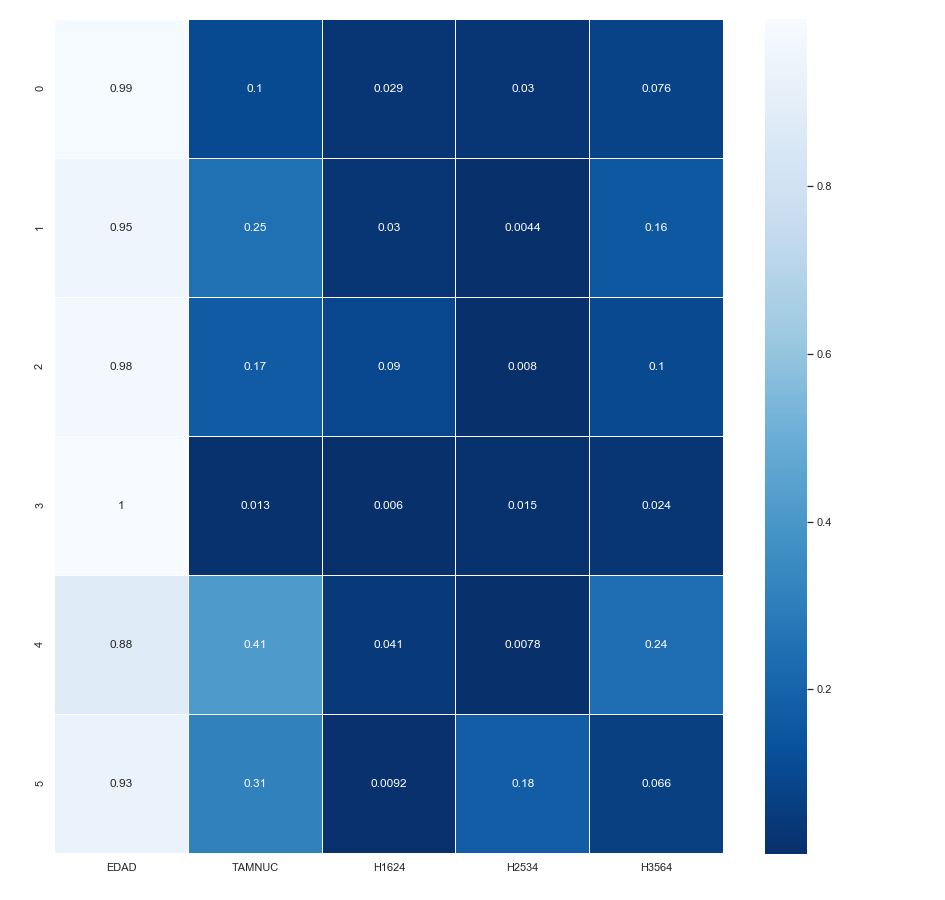
\includegraphics[width=0.9\textwidth]{./imagenes/caso2/heatmap_caso2_K-means}
		\caption{HeatMap usando K-means en el caso de estudio 2.} \label{fig:1}
	\end{figure}

	%------------------------------------------------------------------------

	La figura 2.34 es un dendograma , puede ayudar a decidir el numero de grupos que podrían representar
	mejor la estructura de los datos teniendo en cuenta la forma en la que se van anidando los clusters
	y la medida de similitud a la cual lo hacen. \\

	\begin{figure}[htb]
		\centering
		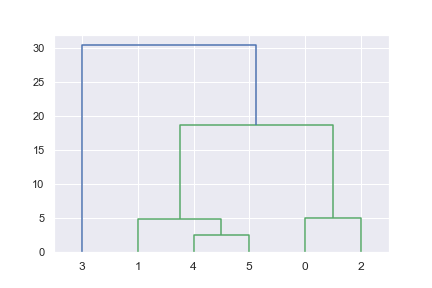
\includegraphics[width=0.6\textwidth]{./imagenes/caso2/dendograma_caso2_K-means}
		\caption{Dendograma usando K-means en el caso de estudio 2.} \label{fig:1}
	\end{figure}

	A continuación se muestra la figura 2.35 , esta es la fusión de las gráficas de 
	Heatmap y de Dendograma.  \\

	\begin{figure}[htb]
		\centering
		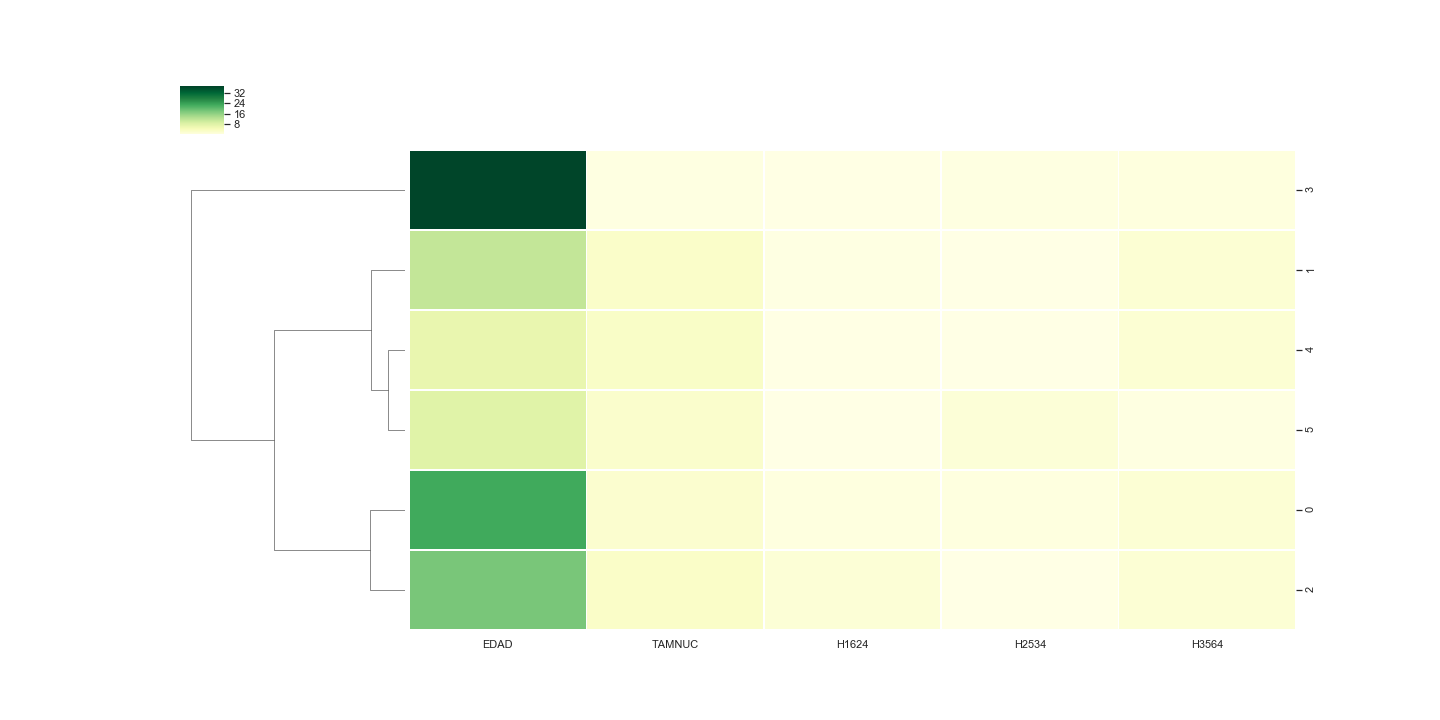
\includegraphics[width=0.9\textwidth]{./imagenes/caso2/heatmapcondendograma_caso2_K-means}
		\caption{HeatMap con Dendograma usando K-means en el caso de estudio 2.} \label{fig:1}
	\end{figure}

	La figura 2.36 esta compuesta por la media de los datos para cada cluster de las variables seleccionadas
	para el estudio. \\ 

	\begin{figure}[htb]
		\centering
		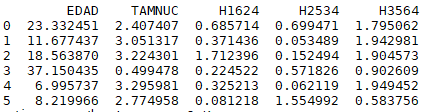
\includegraphics[width=0.6\textwidth]{./imagenes/caso2/medias_datos_caso2_K-means}
		\caption{Medias de los datos seleccionados por cluster K-means.} \label{fig:1}
	\end{figure}

	%----------------------------------------------------------------------
	%							Birch caso 2
	%----------------------------------------------------------------------	

	\subsubsection{Resultados algoritmo Birch caso 2}

	%------------------------------------------------------------------------

	La figura 2.37 representa como están distribuidos los diferentes clusters sobre las diferentes variables estudiadas. (ScatterMatrix)\\

	\begin{figure}[htb]
		\centering
		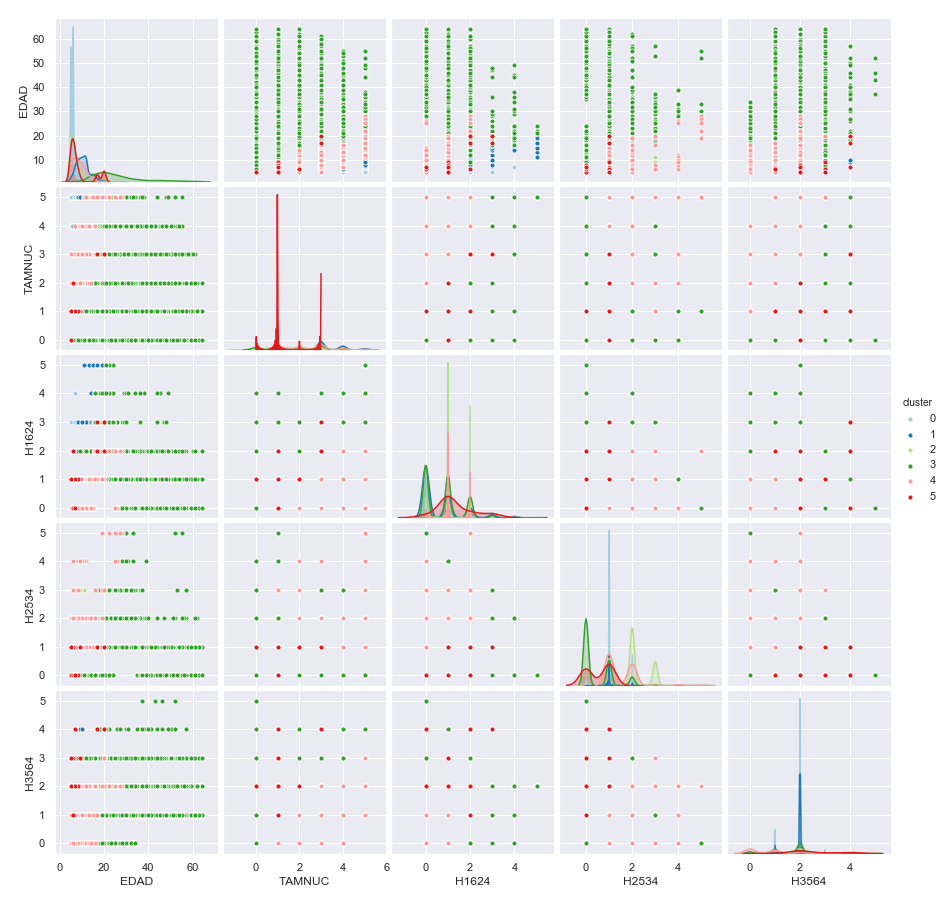
\includegraphics[width=0.9\textwidth]{./imagenes/caso2/scatterMatrix_caso2_Birch}
		\caption{Scatter Matrix usando Birch en el caso de estudio 2.} \label{fig:1}
	\end{figure}
	%------------------------------------------------------------------------

	La figura 2.38 representa la media normalizada de los datos totales de cada variable asociados
	a cada cluster usando el algoritmo Birch para el caso 2.(HeatMap) \\

	\begin{figure}[htb]
		\centering
		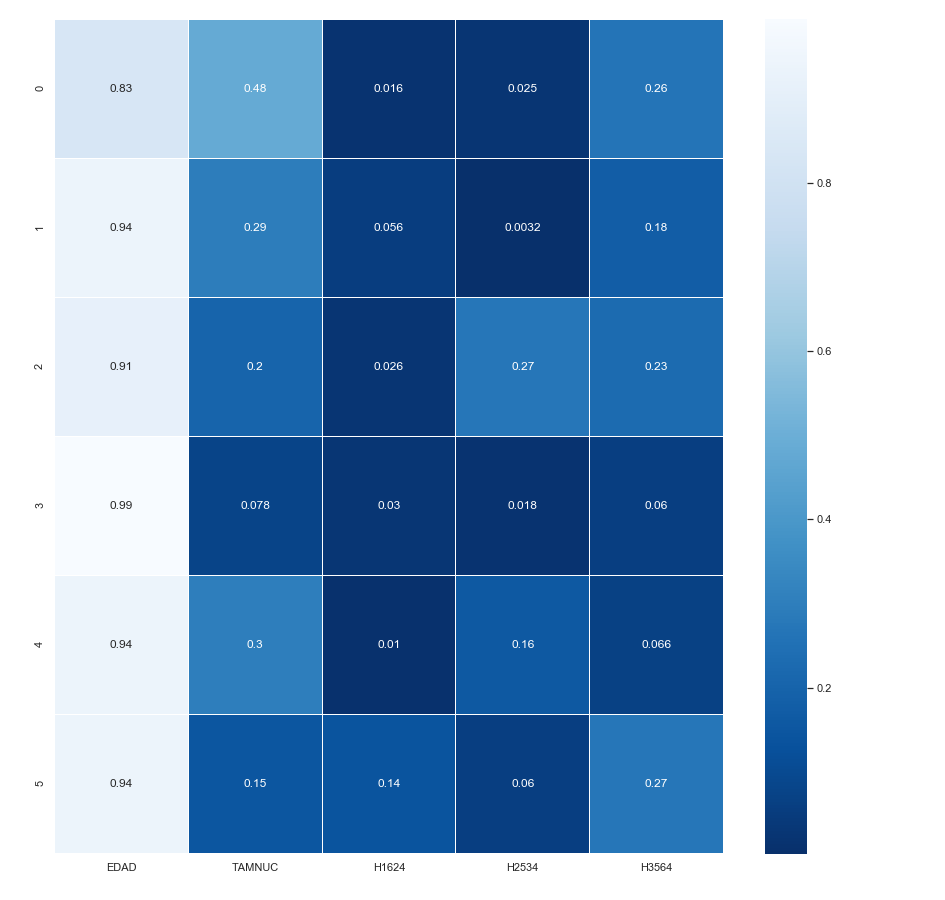
\includegraphics[width=0.9\textwidth]{./imagenes/caso2/heatmap_caso2_Birch}
		\caption{HeatMap usando Birch en el caso de estudio 2.} \label{fig:1}
	\end{figure}

	%------------------------------------------------------------------------

	La figura 2.39 es un dendograma obtenido por la ejecución del algoritmo Birch para
	el caso 2. \\

	\begin{figure}[htb]
		\centering
		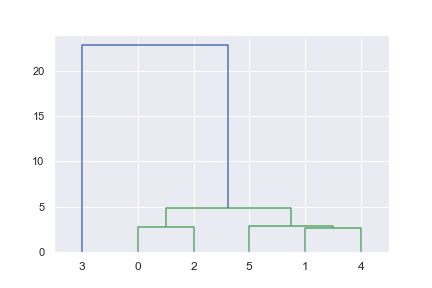
\includegraphics[width=0.6\textwidth]{./imagenes/caso2/dendograma_caso2_Birch}
		\caption{Dendograma usando Birch en el caso de estudio 2.} \label{fig:1}
	\end{figure}

	A continuación se muestra la figura 2.40 , esta es la fusión de las gráficas de 
	Heatmap y de Dendograma.  \\

	\begin{figure}[htb]
		\centering
		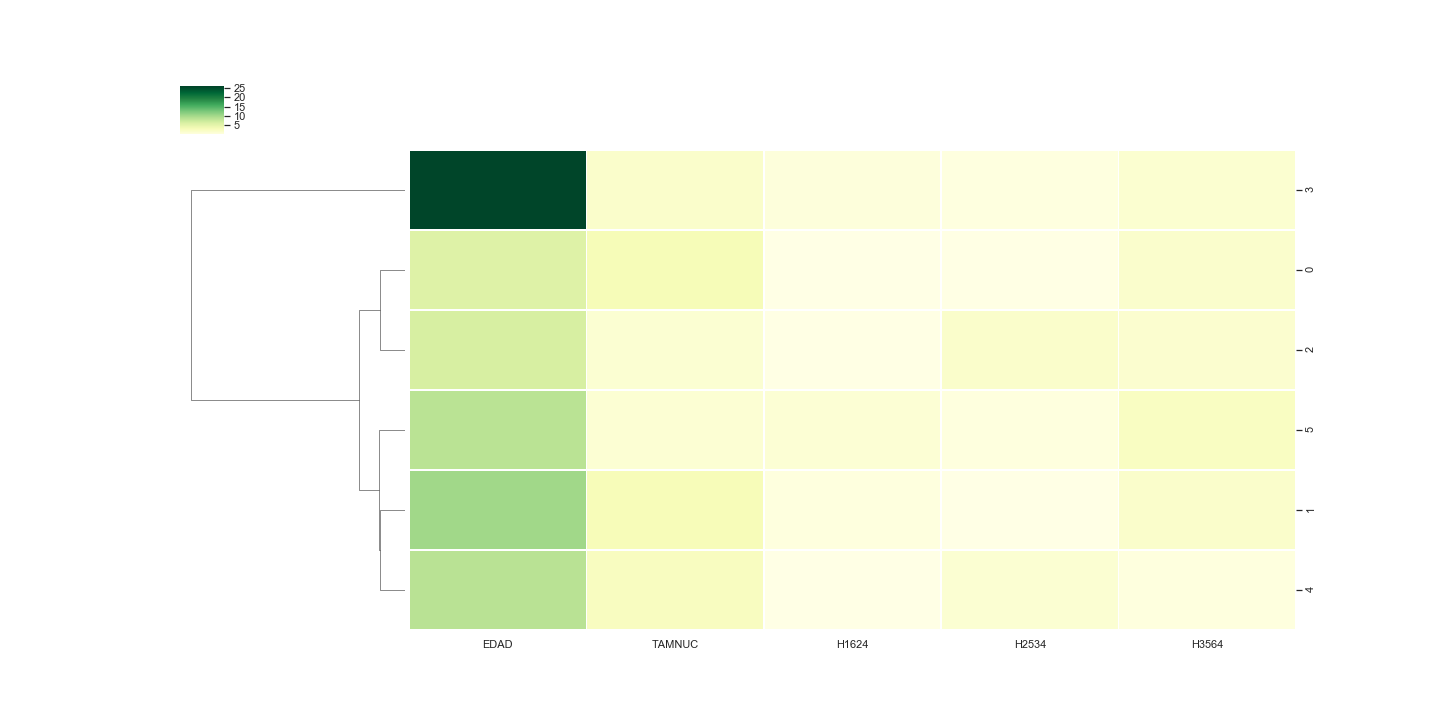
\includegraphics[width=0.9\textwidth]{./imagenes/caso2/heatmapcondendograma_caso2_Birch}
		\caption{HeatMap con Dendograma usando Birch en el caso de estudio 2.} \label{fig:1}
	\end{figure}

	La figura 2.41 esta compuesta por la media de los datos para cada cluster de las variables seleccionadas
	para el estudio 2. \\ 

	\begin{figure}[htb]
		\centering
		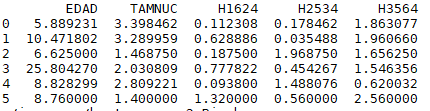
\includegraphics[width=0.6\textwidth]{./imagenes/caso2/medias_datos_caso2_Birch}
		\caption{Medias de los datos seleccionados por cluster Birch caso 2.} \label{fig:1}
	\end{figure}

	%----------------------------------------------------------------------
	%							Ward caso 2
	%----------------------------------------------------------------------	

	\subsubsection{Resultados algoritmo Ward caso 2}

	%------------------------------------------------------------------------

	La figura 2.42 representa como están distribuidos los diferentes clusters sobre las diferentes variables estudiadas
	(Scatter Matrix).\\

	\begin{figure}[htb]
		\centering
		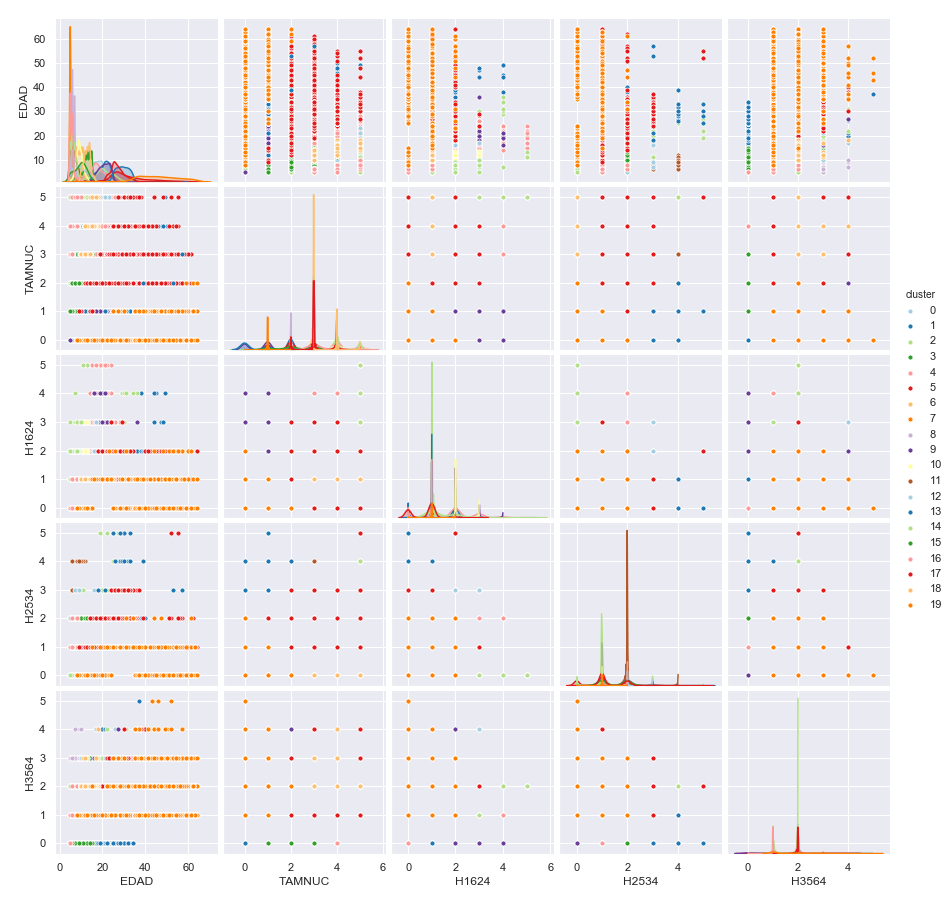
\includegraphics[width=0.9\textwidth]{./imagenes/caso2/scatterMatrix_caso2_Ward}
		\caption{Scatter Matrix usando Ward en el caso de estudio 2.} \label{fig:1}
	\end{figure}
	%------------------------------------------------------------------------

	La figura 2.43 representa la media normalizada de los datos totalas de cada variable asociados
	a cada cluster usando el algoritmo Ward para el caso 2. (HeatMap) \\

	\begin{figure}[htb]
		\centering
		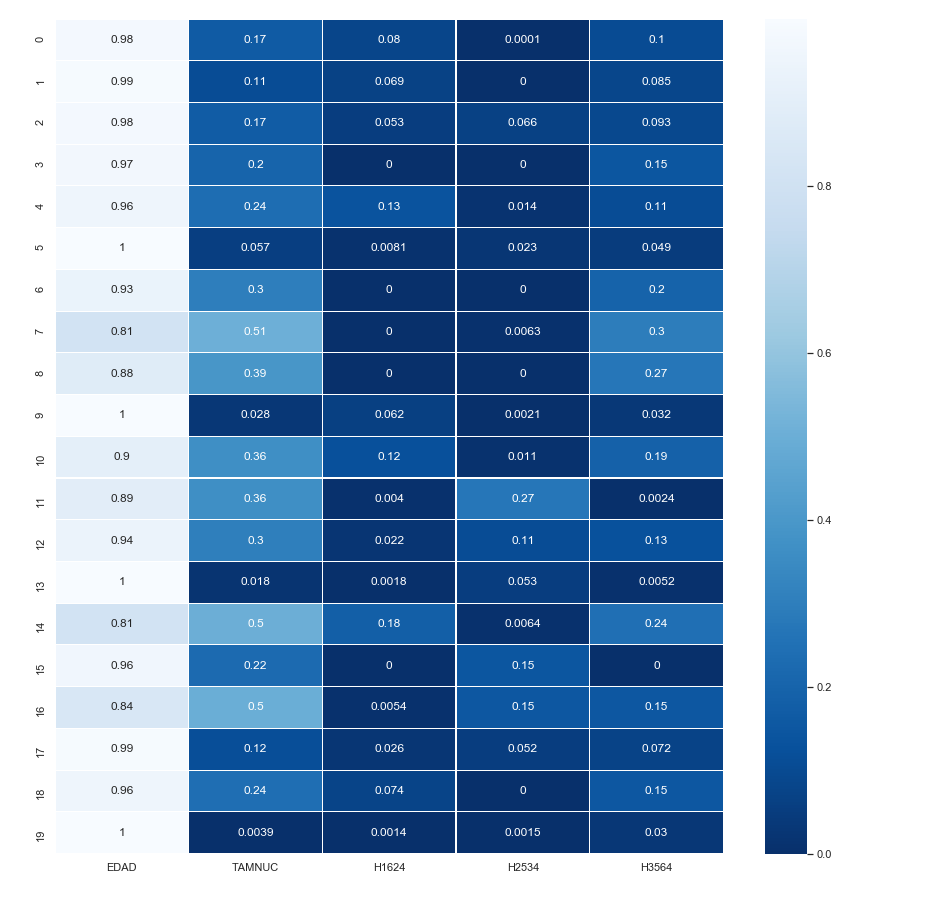
\includegraphics[width=0.9\textwidth]{./imagenes/caso2/heatmap_caso2_Ward}
		\caption{HeatMap usando Ward en el caso de estudio 2.} \label{fig:1}
	\end{figure}

	%------------------------------------------------------------------------

	La figura 2.44 es un dendograma obtenido por la ejecución del algoritmo Ward para
	el caso 2. \\

	\begin{figure}[htb]
		\centering
		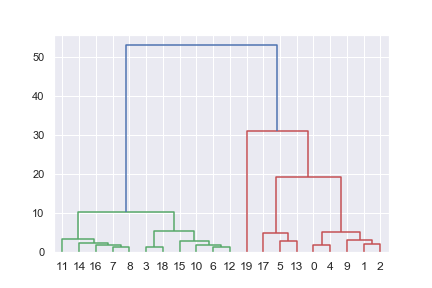
\includegraphics[width=0.6\textwidth]{./imagenes/caso2/dendograma_caso2_Ward}
		\caption{Dendograma usando Ward en el caso de estudio 2.} \label{fig:1}
	\end{figure}

	A continuación se muestra la figura 2.45 , esta es la fusión de las gráficas de 
	Heatmap y de Dendograma.  \\

	\begin{figure}[htb]
		\centering
		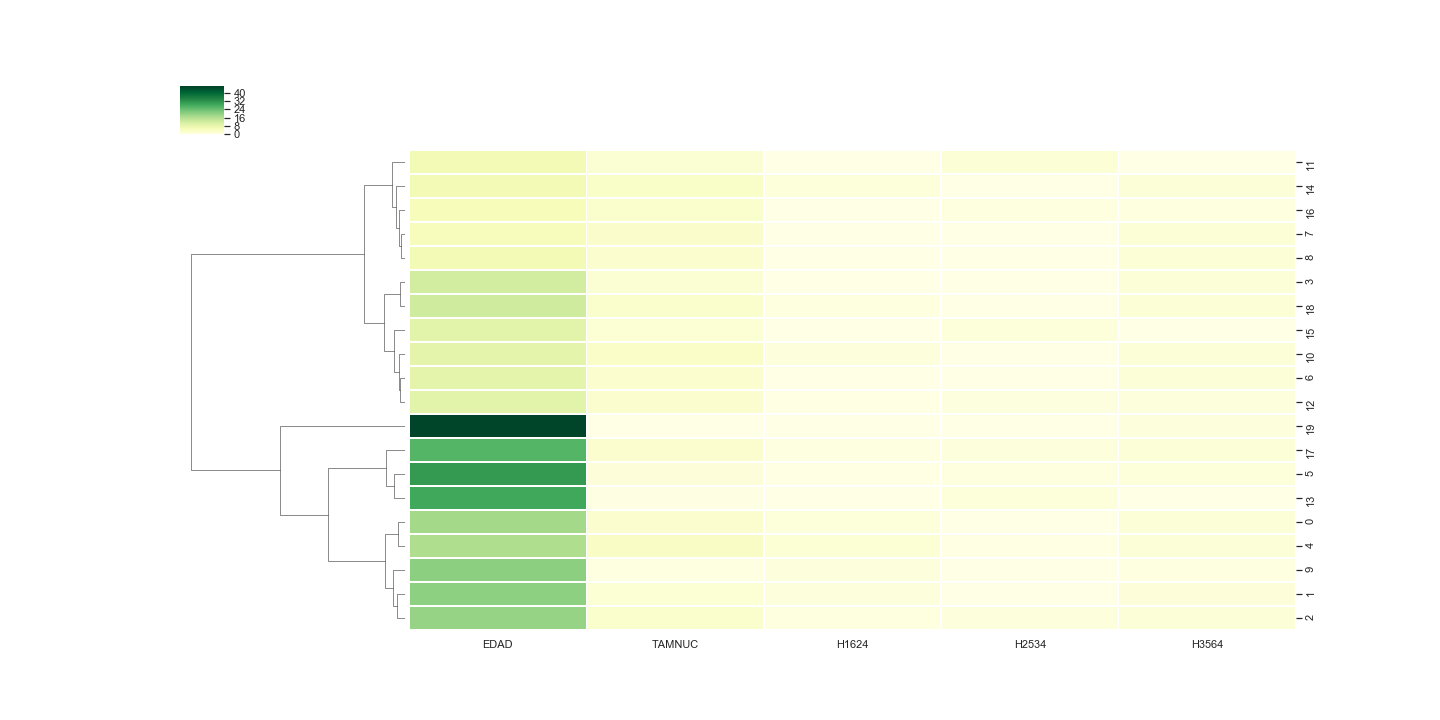
\includegraphics[width=0.9\textwidth]{./imagenes/caso2/heatmapcondendograma_caso2_Ward}
		\caption{HeatMap con Dendograma usando Ward en el caso de estudio 2.} \label{fig:1}
	\end{figure}

	La figura 2.46 esta compuesta por la media de los datos para cada cluster de las variables seleccionadas
	para el estudio del caso 2. \\ 

	\begin{figure}[htb]
		\centering
		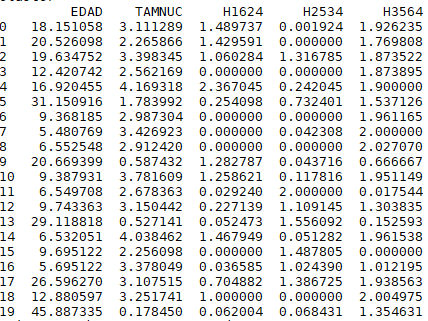
\includegraphics[width=0.6\textwidth]{./imagenes/caso2/medias_datos_caso2_Ward}
		\caption{Medias de los datos seleccionados por cluster Ward caso 2.} \label{fig:1}
	\end{figure}

	%----------------------------------------------------------------------
	%							MeanShift caso 2
	%----------------------------------------------------------------------	

	\subsubsection{Resultados algoritmo MeanShift caso 2}

	%------------------------------------------------------------------------

	La figura 2.47 representa como están distribuidos los diferentes clusters sobre las diferentes variables estudiadas
	(Scatter Matrix).\\

	\begin{figure}[htb]
		\centering
		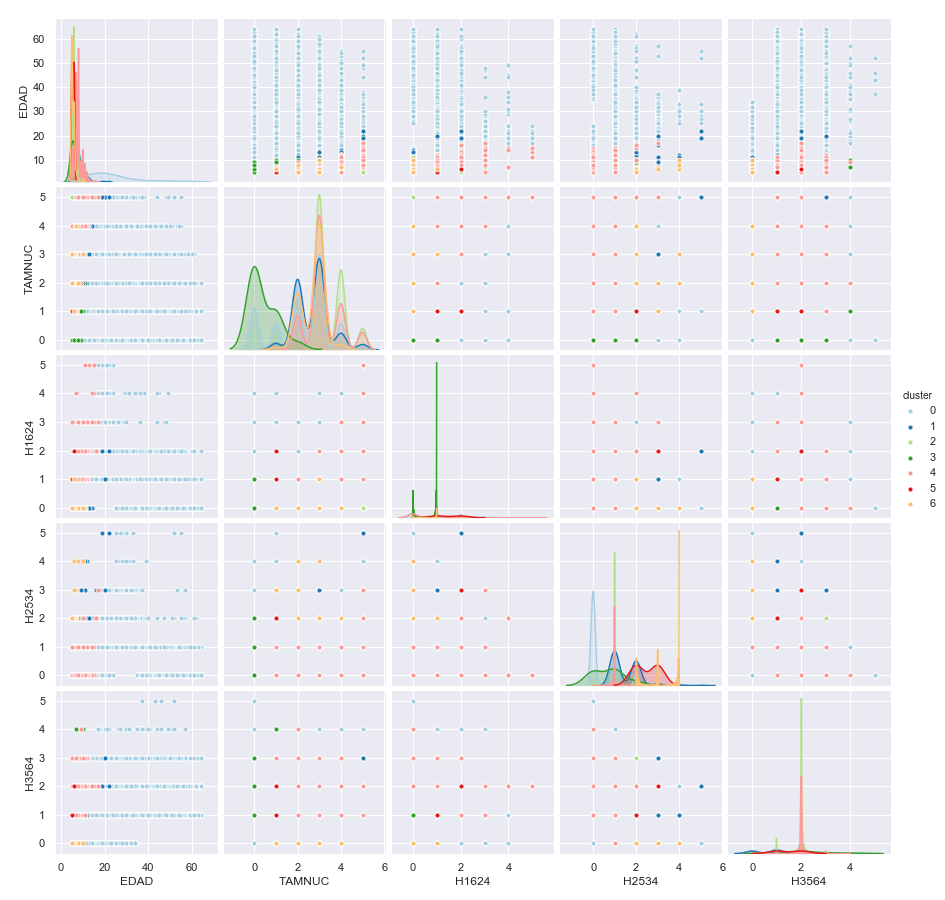
\includegraphics[width=0.9\textwidth]{./imagenes/caso2/scatterMatrix_caso2_MeanShift}
		\caption{Scatter Matrix usando MeanShift en el caso de estudio 2.} \label{fig:1}
	\end{figure}
	%------------------------------------------------------------------------

	La figura 2.48 representa la media normalizada de los datos totales de cada variable asociados
	a cada cluster usando el algoritmo MeanShift para el caso 1. \\

	\begin{figure}[htb]
		\centering
		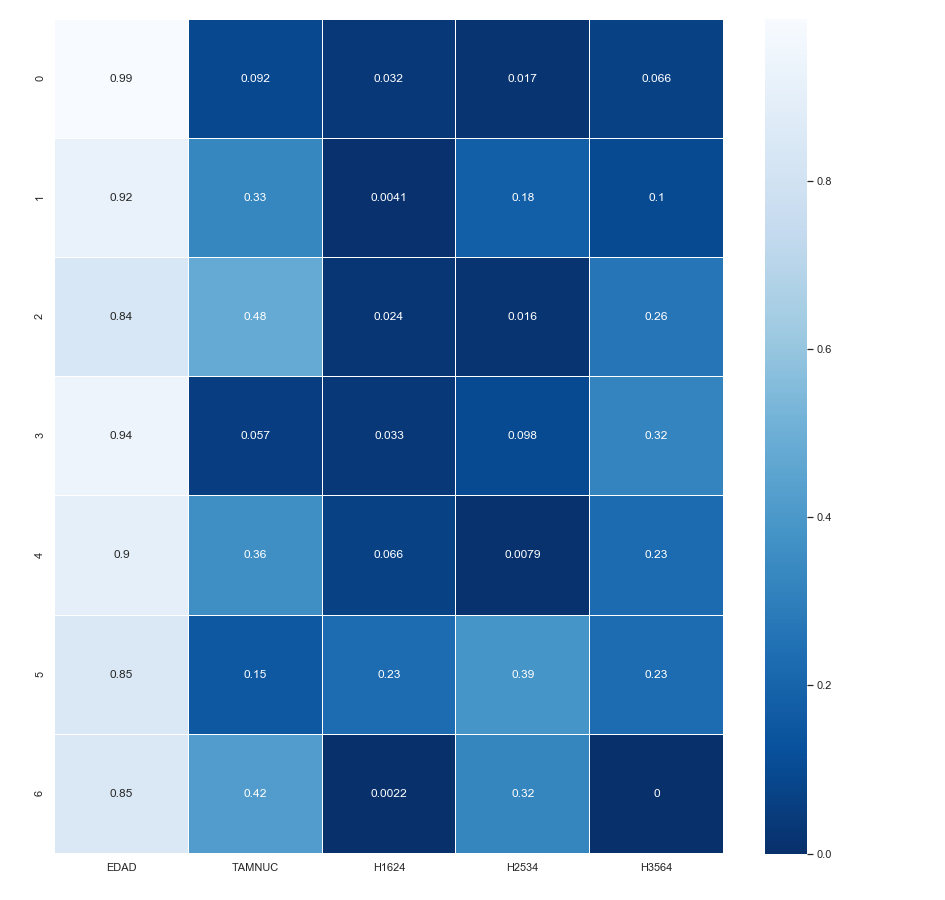
\includegraphics[width=0.9\textwidth]{./imagenes/caso2/heatmap_caso2_MeanShift}
		\caption{HeatMap usando MeanShift en el caso de estudio 2.} \label{fig:1}
	\end{figure}

	%------------------------------------------------------------------------

	La figura 2.49 es un dendograma obtenido por la ejecución del algoritmo MeanShift para
	el caso 2. (HeatMap) \\

	\begin{figure}[htb]
		\centering
		\includegraphics[width=0.6\textwidth]{./imagenes/caso2/dendograma_caso2_MeanShift}
		\caption{Dendograma usando MeanShift en el caso de estudio 2.} \label{fig:1}
	\end{figure}

	A continuación se muestra la figura 2.50 , esta es la fusión de las gráficas de 
	Heatmap y de Dendograma.  \\

	\begin{figure}[htb]
		\centering
		\includegraphics[width=0.9\textwidth]{./imagenes/caso2/heatmapcondendograma_caso2_MeanShift}
		\caption{HeatMap con Dendograma usando MeanShift en el caso de estudio 2.} \label{fig:1}
	\end{figure}

	La figura 2.51 esta compuesta por la media de los datos para cada cluster de las variables seleccionadas
	para el estudio. \\ 

	\begin{figure}[htb]
		\centering
		\includegraphics[width=0.6\textwidth]{./imagenes/caso2/medias_datos_caso2_MeanShift}
		\caption{Medias de los datos seleccionados por cluster MeanShift caso 2.} \label{fig:1}
	\end{figure}

	%----------------------------------------------------------------------
	%							spectral caso 2
	%----------------------------------------------------------------------	

	\subsubsection{Resultados algoritmo Spectral caso 2}

	%------------------------------------------------------------------------

	La figura 2.52 representa como están distribuidos los diferentes clusters sobre las diferentes variables estudiadas
	(Scatter Matrix).\\

	\begin{figure}[htb]
		\centering
		\includegraphics[width=0.9\textwidth]{./imagenes/caso2/scatterMatrix_caso2_spectral}
		\caption{Scatter Matrix usando spectral en el caso de estudio 2.} \label{fig:1}
	\end{figure}
	%------------------------------------------------------------------------

	La figura 2.53 representa la media normalizada de los datos totales de cada variable asociados
	a cada cluster usando el algoritmo spectral para el caso 2. (HeatMap) \\

	\begin{figure}[htb]
		\centering
		\includegraphics[width=0.9\textwidth]{./imagenes/caso2/heatmap_caso2_spectral}
		\caption{HeatMap usando spectral en el caso de estudio 2.} \label{fig:1}
	\end{figure}

	%------------------------------------------------------------------------

	La figura 2.54 es un dendograma obtenido por la ejecución del algoritmo MeanShift para
	el caso 2. \\

	\begin{figure}[htb]
		\centering
		\includegraphics[width=0.6\textwidth]{./imagenes/caso2/dendograma_caso2_spectral}
		\caption{Dendograma usando spectral en el caso de estudio 2.} \label{fig:1}
	\end{figure}

	A continuación se muestra la figura 2.55 , esta es la fusión de las gráficas de 
	Heatmap y de Dendograma.  \\

	\begin{figure}[htb]
		\centering
		\includegraphics[width=1.0\textwidth]{./imagenes/caso2/heatmapcondendograma_caso2_spectral}
		\caption{HeatMap con Dendograma usando spectral en el caso de estudio 2.} \label{fig:1}
	\end{figure}

	La figura 2.56 esta compuesta por la media de los datos para cada cluster de las variables seleccionadas
	para el estudio. \\ 

	\begin{figure}[htb]
		\centering
		\includegraphics[width=0.6\textwidth]{./imagenes/caso2/medias_datos_caso2_spectral}
		\caption{Medias de los datos seleccionados por cluster spectral caso 2.} \label{fig:1}
	\end{figure}

	%----------------------------------------------------------------------
	%						Algoritmos Modificados Caso 2
	%----------------------------------------------------------------------

	\subsubsection[Algoritmos modificados en el caso 2]{Algoritmos modificados en el caso 2}

	En esta sección se va a exponer la modificación de los parámetros de dos algoritmos distintos y para ver sus diferencias
	se van a comparar los resultados de las métricas obtenidas en las secciones previas. \\

	El primer algoritmo que vamos a modificar es Spectral , intentando 
	aumentar el valor de sus métricas aumentando el numero de clusters a 5 a 6 y el segundo algoritmo que vamos a modificar es Ward, 
	y vamos a incrementar su numero de clusters de 20 a 35
	para ver que resultados obtenemos y compararlos con la anterior ejecución. \\

	La figura 2.57 se muestra la antigua tabla pero ahora con las métricas de la ejecucion de estos dos algoritmos modificados.
	En ella se aprecia que las modificaciones de los parámetros no han sido exitosas en ninguno de los casos. 
	En el algoritmo Spectral modificado han disminuido bastante la métrica CH y la métrica SH 
	y en el algoritmo Ward modificado ha disminuido la métrica HC pero ha incrementado un poco la métrica SC. \\

	\begin{figure}[htb]
		\centering
		\includegraphics[width=0.9\textwidth]{./imagenes/caso2/algoritmos_modificados_caso2}
		\caption{Metricas obtenidas usando algoritmos modificados en el caso de estudio 2.} \label{fig:1}
	\end{figure}

	%--------------------------- Spectral -----------------------------------
	\subsubsection{Algoritmo modificado Spectral caso 2} 

	La figura 2.58 representa como están distribuidos los diferentes clusters sobre las diferentes variables con el 
	algoritmo Spectral\\

	\begin{figure}[htb]
		\centering
		\includegraphics[width=0.9\textwidth]{./imagenes/caso2/scatterMatrix_caso2_Spectral_modificado}
		\caption{Scatter Matrix usando Spectral modificado en el caso de estudio 2.} \label{fig:1}
	\end{figure}
	
	A continuación se muestra la figura 2.59 , esta es la fusión de las gráficas de 
	Heatmap y de Dendograma con el algoritmo Spectral modificado.  \\

	\begin{figure}[htb]
		\centering
		\includegraphics[width=1.0\textwidth]{./imagenes/caso2/heatmapcondendograma_caso2_Spectral_modificado}
		\caption{HeatMap con Dendograma usando Spectral modificado en el caso de estudio 2.} \label{fig:1}
	\end{figure}

	%--------------------------- Ward -----------------------------------
	\subsubsection{Algoritmo modificado Ward caso 2}

	La figura 2.60 representa como están distribuidos los diferentes clusters sobre las diferentes variables con el 
	algoritmo Ward modificado\\

	\begin{figure}[htb]
		\centering
		\includegraphics[width=0.9\textwidth]{./imagenes/caso2/scatterMatrix_caso2_Ward_modificado}
		\caption{Scatter Matrix usando Ward modificado en el caso de estudio 2.} \label{fig:1}
	\end{figure}
	
	A continuación se muestra la figura 2.61 , esta es la fusión de las gráficas de 
	Heatmap y de Dendograma con el algoritmo Ward modificado.  \\

	\begin{figure}[htb]
		\centering
		\includegraphics[width=1.0\textwidth]{./imagenes/caso2/heatmapcondendograma_caso2_Ward_modificado}
		\caption{HeatMap con Dendograma usando Ward modificado en el caso de estudio 2.} \label{fig:1}
	\end{figure}

	%----------------------------------------------------------------------
	%					Interpretacion de la segmentacion
	%----------------------------------------------------------------------

	\subsubsection[Interpretacion de la segmentacion caso 2]{Interpretacion de la segmentacion caso 2}

	Para terminar con el estudio de este caso , vamos a interpretar las visualizaciones producidas
	por las ejecuciones de los algoritmos. \\

	Para este caso de estudio, en las gráficas correspondientes a los algoritmos del caso 2
	podemos apreciar que la mayoría de las
	edades de las personas obtenidas con los filtros aplicados  
	oscilan entre 0 y 30 años siendo entre 0 y 20 la parte mayoritaria, con un tamaño familiar de 2 a 4 personas entre las cuales suele haber 
	un miembro entre 16 y 24 años, otro de 25 a 34 y dos miembros de 35 a 64. Son el tipo personas mayormente menores de 25 años que 
	viven con sus dos padres y en ocasiones tienen hermanos.\\

	En el caso del algoritmo Ward podemos ver que en los cluster 3, 6 y 8 se han agrupado aquellas personas
	que no tienen hermanos y solamente viven con sus padres. En los cluster 1 y 18 se han agrupado 
	las personas con algún hermano entre 16 y 24 que viven con sus padres. \\

	Para el caso del algoritmo Spectal , en el cluster cero se agrupan principalmente 
	aquellas personas que viven con varias personas entre 25 y 34 (posiblemente sus padres),
	En los clusters 3 y 4 se agrupan aquellas personas que viven con varias personas entre 35 y 64
	(posiblemente sus padres) y probablemente tengan algún hermano. 

	%----------------------------------------------------------------------
	%							Caso de estudio 3
	%----------------------------------------------------------------------

	\subsection[Caso de estudio 3: Personas solteras mayores de 40 años y sin hijos en el hogar]{Tercer caso de estudio: Personas solteras mayores de 40 años y sin hijos en el hogar}

	En este tercer caso de estudio nos vamos a centrar en aquellas personas solteras mayores de 40 años y sin hijos en el hogar, 
	analizaremos su formación académica y las edades del padre o madre.
	Las variables que vamos a utilizar son : \\

	TESTUD : Tipo de estudios realizados.  \\
	TAMNUC : Tamaño del núcleo familiar . \\
	ESREAL : Estudios realizados. \\
	EDADPAD : Edad del padre. \\
	EDADMAD : Edad de la madre. \\

	En la figura 2.62 se muestran los datos asociados a cada algoritmo usado para este caso de estudio
	de personas que viven con personas mayores , datos como el numero de clusters que se han usado,
	la metrica Calinski-harabasz (CH) , la metrica Siljouette (SC) y el tiempo en segundos que ha tardado
	el algoritmo para ejecutarse . Para este caso de estudio se han contado con un total de 22628 instancias.\\

	\begin{figure}[htb]
		\centering
		\includegraphics[width=0.9\textwidth]{./imagenes/caso3/metricas_algoritmos_caso3}
		\caption{Resultados y caracteristicas de los algoritmos para el caso de estudio 3.} \label{fig:1}
	\end{figure}

	En este caso , vemos como para el indice Calinski-Harabasz los algoritmos con mejor métrica son 
	Ward y K-means, dejando muy por detrás a Birch o MeanShift.  \\

	Para el indice Silhouette no ocurre lo mismo que para el Calinski-Harabasz, ya que todos los resultados se encuentra a la par,
	teniendo MeanShift y Spectral las mejores métricas en este caso. \\

	Por ultimo cabe decir que el algoritmo Spectral es que mayor tiempo de ejecucion tiene. En las siguientes subsecciones
	se muestran gráficas y tablas de algoritmos asociadas a cada algoritmo usado para cada caso de estudio
	, y al final exponemos un análisis de los resultados obtenidos.\\

	Cabe destacar que se ha realizado la eliminación de aquellos clusters con pocos datos (ouliers) . Se ha realizado mediante un 
	filtrado a los clusters con menos de 5 elementos. \\

	%----------------------------------------------------------------------
	%							k-means caso 3
	%----------------------------------------------------------------------	

	\subsubsection{Resultados algoritmo K-Means caso 3}

	%------------------------------------------------------------------------

	La figura 2.63 representa como están distribuidos los diferentes clusters sobre las diferentes variables estudiadas. (Scatter Matrix)\\

	\begin{figure}[htb]
		\centering
		\includegraphics[width=0.9\textwidth]{./imagenes/caso3/scatterMatrix_caso3_K-means}
		\caption{Scatter Matrix usando K-means en el caso de estudio 3.} \label{fig:1}
	\end{figure}
	%------------------------------------------------------------------------

	La figura 2.64 representa la media normalizada de los datos totales de cada variable asociados
	a cada cluster usando el algoritmo k-means para el caso 3. (HeatMap) \\

	\begin{figure}[htb]
		\centering
		\includegraphics[width=0.9\textwidth]{./imagenes/caso3/heatmap_caso3_K-means}
		\caption{HeatMap usando K-means en el caso de estudio 3.} \label{fig:1}
	\end{figure}

	%------------------------------------------------------------------------

	La figura 2.65 es un dendograma , puede ayudar a decidir el numero de grupos que podrían representar
	mejor la estructura de los datos teniendo en cuenta la forma en la que se van anidando los clusters
	y la medida de similitud a la cual lo hacen. \\

	\begin{figure}[htb]
		\centering
		\includegraphics[width=0.6\textwidth]{./imagenes/caso3/dendograma_caso3_K-means}
		\caption{Dendograma usando K-means en el caso de estudio 3.} \label{fig:1}
	\end{figure}

	A continuacion se muestra la figura 2.66 , esta es la fusión de las gráficas de 
	Heatmap y de Dendograma.  \\

	\begin{figure}[htb]
		\centering
		\includegraphics[width=0.9\textwidth]{./imagenes/caso3/heatmapcondendograma_caso3_K-means}
		\caption{HeatMap con Dendograma usando K-means en el caso de estudio 3.} \label{fig:1}
	\end{figure}

	La figura 2.67 esta compuesta por la media de los datos para cada cluster de las variables seleccionadas
	para el estudio. \\ 

	\begin{figure}[htb]
		\centering
		\includegraphics[width=0.6\textwidth]{./imagenes/caso3/medias_datos_caso3_K-means}
		\caption{Medias de los datos seleccionados por cluster K-means.} \label{fig:1}
	\end{figure}

	%----------------------------------------------------------------------
	%							Birch caso 3
	%----------------------------------------------------------------------	

	\subsubsection{Resultados algoritmo Birch caso 3}

	%------------------------------------------------------------------------

	La figura 2.68 representa como están distribuidos los diferentes clusters sobre las diferentes variables estudiadas. (ScatterMatrix)\\

	\begin{figure}[htb]
		\centering
		\includegraphics[width=0.9\textwidth]{./imagenes/caso3/scatterMatrix_caso3_Birch}
		\caption{Scatter Matrix usando Birch en el caso de estudio 3.} \label{fig:1}
	\end{figure}
	%------------------------------------------------------------------------

	La figura 2.69 representa la media normalizada de los datos totales de cada variable asociados
	a cada cluster usando el algoritmo Birch para el caso 3.(HeatMap) \\

	\begin{figure}[htb]
		\centering
		\includegraphics[width=0.9\textwidth]{./imagenes/caso3/heatmap_caso3_Birch}
		\caption{HeatMap usando Birch en el caso de estudio 3.} \label{fig:1}
	\end{figure}

	%------------------------------------------------------------------------

	La figura 2.70 es un dendograma obtenido por la ejecucion del algoritmo Birch para
	el caso 3. \\

	\begin{figure}[htb]
		\centering
		\includegraphics[width=0.6\textwidth]{./imagenes/caso3/dendograma_caso3_Birch}
		\caption{Dendograma usando Birch en el caso de estudio 3.} \label{fig:1}
	\end{figure}

	A continuación se muestra la figura 2.71 , esta es la fusión de las gráficas de 
	Heatmap y de Dendograma.  \\

	\begin{figure}[htb]
		\centering
		\includegraphics[width=0.9\textwidth]{./imagenes/caso3/heatmapcondendograma_caso3_Birch}
		\caption{HeatMap con Dendograma usando Birch en el caso de estudio 3.} \label{fig:1}
	\end{figure}

	La figura 2.72 esta compuesta por la media de los datos para cada cluster de las variables seleccionadas
	para el estudio 3. \\ 

	\begin{figure}[htb]
		\centering
		\includegraphics[width=0.6\textwidth]{./imagenes/caso3/medias_datos_caso3_Birch}
		\caption{Medias de los datos seleccionados por cluster Birch caso 3.} \label{fig:1}
	\end{figure}

	%----------------------------------------------------------------------
	%							Ward caso 3
	%----------------------------------------------------------------------	

	\subsubsection{Resultados algoritmo Ward caso 3}

	%------------------------------------------------------------------------

	La figura 2.73 representa como están distribuidos los diferentes clusters sobre las diferentes variables estudiadas
	(Scatter Matrix).\\

	\begin{figure}[htb]
		\centering
		\includegraphics[width=0.9\textwidth]{./imagenes/caso3/scatterMatrix_caso3_Ward}
		\caption{Scatter Matrix usando Ward en el caso de estudio 3.} \label{fig:1}
	\end{figure}
	%------------------------------------------------------------------------

	La figura 2.74 representa la media normalizada de los datos totales de cada variable asociados
	a cada cluster usando el algoritmo Ward para el caso 3. (HeatMap) \\

	\begin{figure}[htb]
		\centering
		\includegraphics[width=0.9\textwidth]{./imagenes/caso3/heatmap_caso3_Ward}
		\caption{HeatMap usando Ward en el caso de estudio 3.} \label{fig:1}
	\end{figure}

	%------------------------------------------------------------------------

	La figura 2.75 es un dendograma obtenido por la ejecucion del algoritmo Ward para
	el caso 3. \\

	\begin{figure}[htb]
		\centering
		\includegraphics[width=0.6\textwidth]{./imagenes/caso3/dendograma_caso3_Ward}
		\caption{Dendograma usando Ward en el caso de estudio 3.} \label{fig:1}
	\end{figure}

	A continuación se muestra la figura 2.76 , esta es la fusión de las gráficas de 
	Heatmap y de Dendograma.  \\

	\begin{figure}[htb]
		\centering
		\includegraphics[width=0.9\textwidth]{./imagenes/caso3/heatmapcondendograma_caso3_Ward}
		\caption{HeatMap con Dendograma usando Ward en el caso de estudio 3.} \label{fig:1}
	\end{figure}

	La figura 2.77 esta compuesta por la media de los datos para cada cluster de las variables seleccionadas
	para el estudio del caso 3. \\ 

	\begin{figure}[htb]
		\centering
		\includegraphics[width=0.6\textwidth]{./imagenes/caso3/medias_datos_caso3_Ward}
		\caption{Medias de los datos seleccionados por cluster Ward caso 3.} \label{fig:1}
	\end{figure}

	%----------------------------------------------------------------------
	%							MeanShift caso 3
	%----------------------------------------------------------------------	

	\subsubsection{Resultados algoritmo MeanShift caso 3}

	%------------------------------------------------------------------------

	La figura 2.78 representa como están distribuidos los diferentes clusters sobre las diferentes variables estudiadas
	(Scatter Matrix).\\

	\begin{figure}[htb]
		\centering
		\includegraphics[width=0.9\textwidth]{./imagenes/caso3/scatterMatrix_caso3_MeanShift}
		\caption{Scatter Matrix usando MeanShift en el caso de estudio 3.} \label{fig:1}
	\end{figure}
	%------------------------------------------------------------------------

	La figura 2.79 representa la media normalizada de los datos totales de cada variable asociados
	a cada cluster usando el algoritmo MeanShift para el caso 3. \\

	\begin{figure}[htb]
		\centering
		\includegraphics[width=0.9\textwidth]{./imagenes/caso3/heatmap_caso3_MeanShift}
		\caption{HeatMap usando MeanShift en el caso de estudio 3.} \label{fig:1}
	\end{figure}

	%------------------------------------------------------------------------

	La figura 2.80 es un dendograma obtenido por la ejecucion del algoritmo MeanShift para
	el caso 3. (HeatMap) \\

	\begin{figure}[htb]
		\centering
		\includegraphics[width=0.6\textwidth]{./imagenes/caso3/dendograma_caso3_MeanShift}
		\caption{Dendograma usando MeanShift en el caso de estudio 3.} \label{fig:1}
	\end{figure}

	A continuación se muestra la figura 2.81 , esta es la fusión de las gráficas de 
	Heatmap y de Dendograma.  \\

	\begin{figure}[htb]
		\centering
		\includegraphics[width=0.9\textwidth]{./imagenes/caso3/heatmapcondendograma_caso3_MeanShift}
		\caption{HeatMap con Dendograma usando MeanShift en el caso de estudio 3.} \label{fig:1}
	\end{figure}

	La figura 2.82 esta compuesta por la media de los datos para cada cluster de las variables seleccionadas
	para el estudio. \\ 

	\begin{figure}[htb]
		\centering
		\includegraphics[width=0.6\textwidth]{./imagenes/caso3/medias_datos_caso3_MeanShift}
		\caption{Medias de los datos seleccionados por cluster MeanShift caso 2.} \label{fig:1}
	\end{figure}

	%----------------------------------------------------------------------
	%							spectral caso 3
	%----------------------------------------------------------------------	

	\subsubsection{Resultados algoritmo Spectral caso 3}

	%------------------------------------------------------------------------

	La figura 2.83 representa como están distribuidos los diferentes clusters sobre las diferentes variables estudiadas
	(Scatter Matrix).\\

	\begin{figure}[htb]
		\centering
		\includegraphics[width=0.9\textwidth]{./imagenes/caso3/scatterMatrix_caso3_spectral}
		\caption{Scatter Matrix usando spectral en el caso de estudio 3.} \label{fig:1}
	\end{figure}
	%------------------------------------------------------------------------

	La figura 2.84 representa la media normalizada de los datos totales de cada variable asociados
	a cada cluster usando el algoritmo spectral para el caso 3. (HeatMap) \\

	\begin{figure}[htb]
		\centering
		\includegraphics[width=0.9\textwidth]{./imagenes/caso3/heatmap_caso3_spectral}
		\caption{HeatMap usando spectral en el caso de estudio 3.} \label{fig:1}
	\end{figure}

	%------------------------------------------------------------------------

	La figura 2.85 es un dendograma obtenido por la ejecucion del algoritmo MeanShift para
	el caso 3. \\

	\begin{figure}[htb]
		\centering
		\includegraphics[width=0.6\textwidth]{./imagenes/caso3/dendograma_caso3_spectral}
		\caption{Dendograma usando spectral en el caso de estudio 3.} \label{fig:1}
	\end{figure}

	A continuación se muestra la figura 2.86 , esta es la fusión de las gráficas de 
	Heatmap y de Dendograma.  \\

	\begin{figure}[htb]
		\centering
		\includegraphics[width=1.0\textwidth]{./imagenes/caso3/heatmapcondendograma_caso3_spectral}
		\caption{HeatMap con Dendograma usando spectral en el caso de estudio 3.} \label{fig:1}
	\end{figure}

	La figura 2.87 esta compuesta por la media de los datos para cada cluster de las variables seleccionadas
	para el estudio. \\ 
	
	\clearpage

	\begin{figure}[htb]
		\centering
		\includegraphics[width=0.6\textwidth]{./imagenes/caso3/medias_datos_caso3_spectral}
		\caption{Medias de los datos seleccionados por cluster spectral caso 3.} \label{fig:1}
	\end{figure}

	%----------------------------------------------------------------------
	%						Algoritmos Modificados Caso 3
	%----------------------------------------------------------------------

	\subsubsection[Algoritmos modificados en el caso 3]{Algoritmos modificados en el caso 3}

	En esta sección se va a exponer la modificación de los parámetros de dos algoritmos distintos y para ver sus diferencias
	se van a comparar los resultados de las métricas obtenidas en las secciones previas. \\

	El primer algoritmo que vamos a modificar es Birch , intentando 
	aumentar el valor de sus métricas reduciendo el numero de clusters a 10 a 5 y el segundo algoritmo que vamos a modificar es MeanShift, 
	modificando el valor de quantile de 0.4 a 0.2
	para ver que resultados obtenemos y compararlos con la anterior ejecucion. \\

	La figura 2.88 se muestra la antigua tabla pero ahora con las métricas de la ejecucion de estos dos algoritmos modificados.
	En ella se aprecia que las modificaciones de los parámetros no han sido exitosas en el caso del algoritmo Birch, pero si que han incrementado
	un poco la métrica HC del algoritmo MeanShift .\\

	\begin{figure}[htb]
		\centering
		\includegraphics[width=0.9\textwidth]{./imagenes/caso3/algoritmos_modificados_caso3}
		\caption{Metricas obtenidas usando algoritmos modificados en el caso de estudio 3.} \label{fig:1}
	\end{figure}

	%--------------------------- Birch -----------------------------------
	\subsubsection{Algoritmo modificado Birch caso 3} 

	La figura 2.89 representa como están distribuidos los diferentes clusters sobre las diferentes variables con el 
	algoritmo Birch\\

	\begin{figure}[htb]
		\centering
		\includegraphics[width=0.9\textwidth]{./imagenes/caso3/scatterMatrix_caso3_Birch_modificado}
		\caption{Scatter Matrix usando Birch modificado en el caso de estudio 3.} \label{fig:1}
	\end{figure}
	
	A continuación se muestra la figura 2.90 , esta es la fusión de las gráficas de 
	Heatmap y de Dendograma con el algoritmo Birch modificado.  \\

	\begin{figure}[htb]
		\centering
		\includegraphics[width=1.0\textwidth]{./imagenes/caso3/heatmapcondendograma_caso3_Birch_modificado}
		\caption{HeatMap con Dendograma usando Birch modificado en el caso de estudio 3.} \label{fig:1}
	\end{figure}

	%--------------------------- MeanShift -----------------------------------
	\subsubsection{Algoritmo modificado MeanShift caso 3}

	La figura 2.91 representa como están distribuidos los diferentes clusters sobre las diferentes variables con el 
	algoritmo MeanShift modificado\\

	\begin{figure}[htb]
		\centering
		\includegraphics[width=0.9\textwidth]{./imagenes/caso3/scatterMatrix_caso3_MeanShift_modificado}
		\caption{Scatter Matrix usando MeanShift modificado en el caso de estudio 3.} \label{fig:1}
	\end{figure}
	
	A continuación se muestra la figura 2.92 , esta es la fusión de las gráficas de 
	Heatmap y de Dendograma con el algoritmo MeanShift modificado.  \\

	\begin{figure}[htb]
		\centering
		\includegraphics[width=1.0\textwidth]{./imagenes/caso3/heatmapcondendograma_caso3_MeanShift_modificado}
		\caption{HeatMap con Dendograma usando MeanShift modificado en el caso de estudio 3.} \label{fig:1}
	\end{figure}

	%----------------------------------------------------------------------
	%					Interpretacion de la segmentacion
	%----------------------------------------------------------------------

	\subsubsection[Interpretacion de la segmentacion caso 3]{Interpretacion de la segmentacion caso 3}

	Para terminar con el estudio de este caso , vamos a interpretar las visualizaciones producidas
	por las ejecuciones de los algoritmos. \\

	Para este caso de estudio, en las gráficas correspondientes a los algoritmos del caso 3
	podemos apreciar que las edades de los padres y las madres , como es normal , se asemejan mucho,
	estando en el rango 60 - 90 . También hay personas que no viven con sus padres, en el scatterMatrix
	tienen el valor 0 porque en el pre procesado se puso este valor a todos los huecos vacíos, que en nuestro caso 
	son personas que no conviven con su padre o madre. El tamaño del núcleo familiar no supera las dos personas , \\

	En el caso del algoritmo K-means podemos ver como en los clusters 0 t 9 se han agrupado aquellas personas que 
	tienen muchos valores 0 en sus atributos, tanto en la edad del padre y madre, que significa que no convive
	con ellos , como en el tipo de estudios , que quiere decir que tiene unos estudios realizados
	con un valor de 5 o menos , tres en nuestro caso , que significa que fueron mas de 5 años a la
	escuela pero no acabaron sus estudios primarios. En el cluster 8 tenemos aquellas personas
	con una licenciatura, arquitectura ,ingeniería o doctorado que no viven con su padre y su madre.\\

	%----------------------------------------------------------------------
	%							Bibliografia
	%----------------------------------------------------------------------

	\section[Bibliografía]{Bibliografía.}
	
	\begin{thebibliography}{99}
		%---------------------------------------
		\bibitem{cite1} 
		\textsc{Instituto Nacional de Estadistica}
		\newline
		\url{http://www.ine.es/censos2011_datos/cen11_datos_microdatos.htm}	
		%---------------------------------------
		\bibitem{cite2} 
		\textsc{Python ORG}
		\newline
		\url{https://www.python.org/downloads/release/python-370/}	
		%---------------------------------------
		\bibitem{cite3} 
		\textsc{K-means}
		\newline
		\url{https://www.datascience.com/blog/k-means-clustering}
		%---------------------------------------
		\bibitem{cite5} 
		\textsc{Spectral Clustering}
		\newline
		\url{https://scikit-learn.org/stable/modules/generated/sklearn.cluster.SpectralClustering.html}
		%---------------------------------------
		\bibitem{cite6} 
		\textsc{Mean Shift}
		\newline
		\url{https://scikit-learn.org/stable/modules/generated/sklearn.cluster.MeanShift.html}
		%---------------------------------------
		\bibitem{cite7} 
		\textsc{Ward}
		\newline
		\url{https://scikit-learn.org/stable/modules/clustering.html}
		%---------------------------------------
		\bibitem{cite9} 
		\textsc{Birch}
		\newline
		\url{https://scikit-learn.org/stable/modules/clustering.html}
	\end{thebibliography}


\end{document}